\documentclass[a4paper]{article}
\usepackage[danish]{babel}
\usepackage{amsfonts, amssymb, mathtools, amsthm, amsmath}
\usepackage{graphicx, pgfplots}
\usepackage{url}
\usepackage[dvipsnames]{xcolor}
\usepackage{lastpage}
\usepackage{multicol} 

%loaded last
\usepackage[hidelinks]{hyperref}
\usepackage{bookmark} 

\usepackage{siunitx}
  \sisetup{exponent-product = \cdot,
    output-decimal-marker = {,}}

%Giles Castelles incfig
\usepackage{import}
\usepackage{xifthen}
\usepackage{pdfpages}
\usepackage{transparent}

\newcommand{\incfig}[2][1]{%
  \def\svgwidth{#1\columnwidth}
  \import{./figures/}{#2.pdf_tex}
}

\setlength{\oddsidemargin}{0in}
\setlength{\textwidth}{6.5in}
\setlength{\textheight}{8.8in}
\setlength{\topmargin}{0in}
\setlength{\headheight}{18pt}
\setlength{\parindent}{0pt}
\setlength{\parskip}{0.5\baselineskip}

\usepackage{fancyhdr}
\pagestyle{fancy}

\fancyhead{}
\fancyfoot{}
\fancyfoot[R]{\thepage}
\fancyhead[C]{\leftmark}

\pgfplotsset{compat=newest}

\pgfplotsset{every axis/.append style={
  axis x line=middle,    % put the x axis in the middle
  axis y line=middle,    % put the y axis in the middle
  axis line style={<->,color=black}, % arrows on the axis
}}

\usepackage{thmtools}
\usepackage{tcolorbox}
  \tcbuselibrary{skins, breakable}
  \tcbset{
    space to upper=1em,
    space to lower=1em,
  }

\theoremstyle{definition}

\newtcolorbox[auto counter]{definition}[1][]{%
  breakable,
  colframe=ForestGreen,  %frame color
  colback=ForestGreen!5, %background color
  colbacktitle=ForestGreen!25, %background color for title
  coltitle=ForestGreen!70!black,  %title color
  fonttitle=\bfseries\sffamily, %title font
  left=1em,              %space on left side in box,
  enhanced,              %more options
  frame hidden,          %hide frame
  borderline west={2pt}{0pt}{ForestGreen},  %display left line
  title=Definition \thetcbcounter: #1,
}

\newtcolorbox{greenline}{%
  breakable,
  colframe=ForestGreen,  %frame color
  colback=white,          %remove background color
  left=1em,              %space on left side in box
  enhanced,              %more options
  frame hidden,          %hide frame
  borderline west={2pt}{0pt}{ForestGreen},  %display left line
}

\newtcolorbox[auto counter, number within=section]{eks}[1][]{%
  breakable,
  colframe=NavyBlue,  %frame color
  colback=NavyBlue!5, %background color
  colbacktitle=NavyBlue!25,    %background color for title
  coltitle=NavyBlue!70!black,  %title color
  fonttitle=\bfseries\sffamily, %title font
  left=1em,            %space on left side in box,
  enhanced,            %more options
  frame hidden,        %hide frame
  borderline west={2pt}{0pt}{NavyBlue},  %display left line
  title=Eksempel \thetcbcounter: #1
}

\newtcolorbox{blueline}{%
  breakable,
  colframe=NavyBlue,     %frame color
  colback=white,         %remove background
  left=1em,              %space on left side in box,
  enhanced,              %more options
  frame hidden,          %hide frame
  borderline west={2pt}{0pt}{NavyBlue},  %display left line
}

\newtcolorbox{teo}[1][]{%
  breakable,
  colframe=RawSienna,  %frame color
  colback=RawSienna!5, %background color
  colbacktitle=RawSienna!25,    %background color for title
  coltitle=RawSienna!70!black,  %title color
  fonttitle=\bfseries\sffamily, %title font
  left=1em,              %space on left side in box,
  enhanced,              %more options
  frame hidden,          %hide frame
  borderline west={2pt}{0pt}{RawSienna},  %display left line
  title=Teori: #1,
}

\newtcolorbox[auto counter, number within=section]{sæt}[1][]{%
  breakable,
  colframe=RawSienna,  %frame color
  colback=RawSienna!5, %background color
  colbacktitle=RawSienna!25,    %background color for title
  coltitle=RawSienna!70!black,  %title color
  fonttitle=\bfseries\sffamily, %title font
  left=1em,              %space on left side in box,
  enhanced,              %more options
  frame hidden,          %hide frame
  borderline west={2pt}{0pt}{RawSienna},  %display left line
  title=Sætning \thetcbcounter: #1,
  before lower={\textbf{Bevis:}\par\vspace{0.5em}},
  colbacklower=RawSienna!25,
}

\newtcolorbox{redline}{%
  breakable,
  colframe=RawSienna,  %frame color
  colback=white,       %Remove background color
  left=1em,            %space on left side in box,
  enhanced,            %more options
  frame hidden,        %hide frame
  borderline west={2pt}{0pt}{RawSienna},  %display left line
}

\newtcolorbox{for}[1][]{%
  breakable,
  colframe=NavyBlue,  %frame color
  colback=NavyBlue!5, %background color
  colbacktitle=NavyBlue!25,    %background color for title
  coltitle=NavyBlue!70!black,  %title color
  fonttitle=\bfseries\sffamily, %title font
  left=1em,              %space on left side in box,
  enhanced,              %more options
  frame hidden,          %hide frame
  borderline west={2pt}{0pt}{NavyBlue},  %display left line
  title=Forklaring #1,
}

\newtcolorbox{bem}{%
  breakable,
  colframe=NavyBlue,  %frame color
  colback=NavyBlue!5, %background color
  colbacktitle=NavyBlue!25,    %background color for title
  coltitle=NavyBlue!70!black,  %title color
  fonttitle=\bfseries\sffamily, %title font
  left=1em,              %space on left side in box,
  enhanced,              %more options
  frame hidden,          %hide frame
  borderline west={2pt}{0pt}{NavyBlue},  %display left line
  title=Bemærkning:,
}

\makeatother
\def\@lecture{}%
\newcommand{\lecture}[3]{
  \ifthenelse{\isempty{#3}}{%
    \def\@lecture{Lecture #1}%
  }{%
    \def\@lecture{Lecture #1: #3}%
  }%
  \subsection*{\makebox[\textwidth][l]{\@lecture \hfill \normalfont\small\textsf{#2}}}
}

%Format lim the same way in intext and in display
\let\svlim\lim\def\lim{\svlim\limits}

% horizontal rule
\newcommand\hr{
\noindent\rule[0.5ex]{\linewidth}{0.5pt}
}

\author{Noah Rahbek Bigum Hansen}

\title{Fysik og Mekanik – formelsamling}
\date{Efteråret 2024}
\begin{document}
    \maketitle
    \tableofcontents
    \newpage
    \section{Enheder, fysiske størrelser og vektorer}

\subsection{Vektorprodukter (1.10)}

\subsubsection{Skalarproduktet}
Lad $\Vec{A}$ og $\Vec{B}$ være to vektorer. Prikproduktet $\Vec{A} \cdot \Vec{B}$ er da defineret som
\[
\Vec{A} \cdot \Vec{B} = AB \cos\phi = \left| \Vec{A} \right| \left| \Vec{B} \right| \cos\phi
\]
Hvor $A$ og $|\Vec{A}|$ er størrelsen af $\Vec{A}$, $B$ og $\Vec{B}$ er størrelsen af $\Vec{B}$ og $\phi$ er vinklen mellem de to vektorer, hvis de lægges så deres ``startpunkter'' er sammenfaldende. For $\ang{0} < \phi < \ang{90}$ er skalarproduktet positivt mens det for $\ang{90} < \phi < \ang{180}$ er negativt -- for $\phi = \ang{90}$ er skalaproduktet 0. 

Skalarproduktet kan også skrives som
\[ 
\Vec{A} \cdot \Vec{B} = A_xB_x + A_yB_y + A_zB_z
.\]
Hvor $\Vec{A} = (A_x, A_y, A_y)$ og $\Vec{B} = (B_x, B_y, B_z)$.

\subsubsection{Krydsproduktet}
Lad $\Vec{A}$ og $\Vec{B}$ være to vektorer. Krydsproduktet $\Vec{A} \times \Vec{B}$ er da defineret som
\[ 
\left| \Vec{C} \right| = \left| \Vec{A} \right| \left| \Vec{B} \right| \sin\phi 
.\]
Hvor $\left| \Vec{C} \right|$ er længden af den resulterende vektor som fås fra krydsproduktet. $\left| \Vec{A} \right|$ og $\left| \Vec{B} \right|$ er længden af hhv. $\Vec{A}$ og $\Vec{B}$ mens $\phi$ er vinklen mellem de to vektorer, hvis de lægges så deres ``startpunkter'' er sammenfaldende. 

Komposanterne til den resulterende vektor af krydsproduktet $\Vec{C} = (C_x, C_y, C_z)$ kan findes som
\[ 
C_x = A_yB_z - A_zB_y, \quad C_y = A_zB_z - A_xB_z, \quad C_z = A_xB_y - A_yB_x
.\]
Hvor $\Vec{A} = (A_x, A_y, A_y)$ og $\Vec{B} = (B_x, B_y, B_z)$.

    \newpage
    \section{Bevægelse langs en ret linje}

\begin{table}[ht]
\begin{tabular}{|l|l|l|}
\hline
\textbf{Givet}                                            & \textbf{Ønsker at finde} & \textbf{Relevante formler} \\ \hline
Strækning og tid & Hastighed    & \begin{tabular}[c]{@{}l@{}}\ref{afs:gnshas} – Gennemsnitlig hastighed\\ \ref{afs:inshas} – Øjeblikshastighed\end{tabular}       \\ \hline
Hastighed og tid & Acceleration & \begin{tabular}[c]{@{}l@{}}\ref{afs:gnsacc} – Gennemsnitlig acceleration\\ \ref{afs:insacc} – Øjebliksacceleration\end{tabular} \\ \hline
Konstant acceleration, starthastighed, tid                & Sluthastighed            & \ref{afs:velconacc}        \\ \hline
Konstant acceleration, tid, starthastighed, startposition & Slutposition             & \ref{afs:posconacc}        \\ \hline
Acceleration, starthastighed, tid                         & Sluthastighed            & \ref{afs:hasacc}           \\ \hline
Hastighed, startposition, tid                             & Slutposition             & \ref{afs:poshas}           \\ \hline
\end{tabular}
\end{table}


\subsection{Strækning, tid og hastighed (2.1-2)}

\subsubsection{Gennemsnitlig hastighed} \label{afs:gnshas}
Den gennemsnitlige hastighed er givet som ændringen i strækning $\Delta x = x_2 - x_1$ over ændringen i tid $\Delta t = t_2 - t_1$. Altså har vi at
\[ 
v_{av_x} = \frac{\Delta x}{\Delta t} = \frac{x_2 - x_1}{t_2 - t_1}
.\]

\subsubsection{Øjeblikshastighed (Eng: \textit{Instantaneous velocity})} \label{afs:inshas} 
Øjeblikshastigheden i $x$-retningen $v_x$ er givet ved den gennemsnitlige hastighed når $\Delta \to 0$. Altså
\[ 
v_x = \lim_{\Delta t \to 0} \frac{\Delta x}{\Delta t} = \frac{\mathrm{d}x}{\mathrm{d}t}
.\]

\subsection{Acceleration (2.3)}

\subsubsection{Gennemsnitlig acceleration} \label{afs:gnsacc}
Vi betragter en partikel der bevæger sig langs $x$-aksen. Lad $P_1$ angive et punkt hvor partiklen har hastighed $v_{1x}$ til tiden $t_1$ og $P_2$ angive et tilsvarende punkt hvor partiklen istedet har hastigheden $v_{2x}$ til tiden $t_2$. Idet partiklen bevæger sig fra $P_1$ til $P_2$ på $\Delta t = t_2 - t_1$ og ændrer sin hastighed med $\Delta v_x = v_{2x} - v_{1x}$ så er den gennemsnitlige acceleration givet som
\[ 
a_{av_x} = \frac{\Delta v_x}{\Delta t} = \frac{v_{2x} - v_{1x}}{t_2 - t_1}
.\]

\subsubsection{Øjebliksacceleration (Eng: \textit{Instantaneous acceleration})} \label{afs:insacc}
Øjebliksaccelerationen i $x$-retningen $a_x$ er defineret som den gennemsnitlige acceleration når $\Delta t \to 0$. Altså
\[ 
a_x = \lim_{\Delta t \to 0} \frac{\Delta v_x}{\Delta t} = \frac{\mathrm{d}v_x}{\mathrm{d}t}
.\]


\subsection{Bevægelse med konstant acceleration}

\subsubsection{Hastighed ved konstant acceleration} \label{afs:velconacc}
Vi betragter en partikel, der bevæger sig langs x-aksen. Lad $v_{0x}$ være partiklens hastighed til $t = 0$, $a_x$ være partiklens \textit{konstante} acceleration og $t$ være tiden. Hastigheden i $x$-retningen $v_x$ til tiden $t$ er da givet som
\[ 
v_x = v_{0x} + a_xt
.\]

Har man i stedet fået givet to punkter $x$ og $x_0$ men ingen tid $t$ kan følgende formel benyttes i stedet
\[ 
v_x^2 = v_{0x}^2 + 2a_x(x-x_0)
.\]


\subsubsection{Position ved konstant acceleration} \label{afs:posconacc}
Vi betragter en partikel, der bevæger sig langs x-aksen. Lad $x_0$ være partiklens position til $t = 0$, $v_{0x}$ være partiklens hastighed til $t = 0$, $a_x$ være partiklens \textit{konstante} acceleration og $t$ være tiden. Positionen af partiklen til tiden $t$ er da givet som
\[ 
x = x_0 + v_{0x}t + \frac{1}{2}a_xt^2
.\]

Har man ikke fået opgivet den konstante acceleration $a_x$ men i stedet en start og en sluthastighed $v_{0x}$ og $v_x$ kan følgende formel benyttes
\[ 
x-x_0 = \frac{1}{2}(v_{0x} + v_x)t
.\]
Her er det værd at bemærke at formlen ovenfor kun kan benyttes for konstant acceleration, dette gælder selvom denne acceleration ikke er givet.


\subsection{Hastighed og position ved integration (2.6)}

\subsubsection{Hastighed som integralet af acceleration} \label{afs:hasacc}
Har man fået oplyst en funktion $a_x$ der beskriver accelerationen som funktion af tid samt en initialhastighed $v_{0x}$ kan hastigheden $v_x$ til tiden $t$ findes som
\[ 
v_x = v_{0x} + \int_{0}^{t} a_x \, \mathrm{d}t 
.\]


\subsubsection{Position som integralet af hastighed} \label{afs:poshas}
Har man fået oplyst en funktion $v_x$ der beskriver hastigheden som funktion af tid samt en initialposition $x_{0}$ kan positionen $x$ til tiden $t$ findes som
\[ 
x = x_0 + \int_{0}^{t} v_x \, \mathrm{d}t 
.\]


    \newpage
    \section{Bevægelse i to eller tre dimensioner}

\begin{table}[ht]
\begin{tabular}{|l|l|l|}
\hline
\textbf{Givet}                      & \textbf{Ønsker at finde} & \textbf{Relevante formler} \\ \hline
Strækning og tid & Hastighed    & \begin{tabular}[c]{@{}l@{}}\ref{afs:gnshasvec} – Gennemsnitlig hastighed\\ \ref{afs:inshasvec} – Øjeblikshastighed\end{tabular}       \\ \hline
Hastighed og tid & Acceleration & \begin{tabular}[c]{@{}l@{}}\ref{afs:gnsacc} – Gennemsnitlig acceleration\\ \ref{afs:insacc} – Øjebliksacceleration\end{tabular}       \\ \hline
Hastighed                           & Hastighedskomposanter    & \ref{afs:haskom}           \\ \hline
Hastighedskomposanter               & Hastighed                & \ref{afs:komhas}           \\ \hline
Hastighed, tid   & acceleration & \begin{tabular}[c]{@{}l@{}}\ref{afs:gnsaccvec} – Gennemsnitlig acceleration\\ \ref{afs:insaccvec} – Øjebliksacceleration\end{tabular} \\ \hline
Acceleration                        & Accelerationskomposanter & \ref{afs:acckom}           \\ \hline
Accelerationskomposanter            & Acceleration             & \ref{afs:komacc}           \\ \hline
Kastevinkel, starthastighed, tid    & Kasteafstand             & \ref{afs:kasafs}           \\ \hline
Starthastighed, kastevinkel, tid    & Kastehøjde               & \ref{afs:kashøj}           \\ \hline
Starthastighed, kastevinkel         & Horisontal hastighed     & \ref{afs:kashhas}          \\ \hline
Starthastighed, kastevinkel, tid    & Vertikal hastighed       & \ref{afs:kasvhas}          \\ \hline
Hastighed, radius                   & Centripetalacceleration  & \ref{afs:acccp}            \\ \hline
Hastighed ift. to referencesystemer & Relativ hastighed        & \ref{afs:hastrans}         \\ \hline
\end{tabular}
\end{table}

\subsection{Hastighedsvektorer (3.1)}

\subsubsection{Gennemsnitshastigshedsvektor (Eng: \textit{Average velocity vector})} \label{afs:gnshasvec}
På samme måde som i \textbf{\ref{afs:gnshas}: \nameref{afs:gnshas}} kan vi finde gennemsnitshastighedsvektoren $\Vec{v_{av}}$ som kvotienten mellem ændringen i positionsvektoren $\Delta \Vec{r}$ og ændringen i tid $\Delta t$. Altså
\[ 
\Vec{v}_{\text{av}} = \frac{\Delta \Vec{r}}{\Delta t} = \frac{\Vec{r_2} - \Vec{r_1}}{t_2 - t_1}
.\]


\subsubsection{Øjeblikshastighedsvektor (Eng: \textit{instantaneous velocity vector})} \label{afs:inshasvec}
På samme måde som i \ref{afs:inshas}: \nameref{afs:inshas} kan vi finde øjeblikshastighedsvektoren $\Vec{v}$ som kvotienten mellem ændringen i positionsvektoren $\Delta \Vec{r}$ og ændringen i tid $\Delta t$ når $\Delta t \to 0$. Altså
\[ 
\Vec{v} = \lim_{\Delta t \to 0} \frac{\Delta \Vec{r}}{\Delta t} = \frac{\mathrm{d}\Vec{r}}{\mathrm{d}t}
.\]

\subsubsection{Hastighedskomposanter} \label{afs:haskom}
Hastigheden i en given retning er blot ændringen i position i denne retning over tid. Altså
\[ 
  v_x = \frac{\mathrm{d}x}{\mathrm{d}t}, v_y = \frac{\mathrm{d}y}{\mathrm{d}t}, v_z = \frac{\mathrm{d}z}{\mathrm{d}t}
.\]

\subsubsection{Størrelsen af hastighedsvektoren fra komposanter} \label{afs:komhas}
Givet størrelen på komposanterne,($v_x, v_y, v_z)$ til hastighedsvektoren $\Vec{v}$ kan størrelsen af hastighedsvektoren $\left| \Vec{v} \right|$ findes med Pythagoras som
\[
\left| \Vec{v} \right| = \sqrt{v_x^2 + v_y^2 + v_z^2}
.\]



\subsection{Accelerationsvektorer (3.2)}
\subsubsection{Gennemsnitsaccelerationsvektor (Eng: \textit{Average acceleration vector})} \label{afs:gnsaccvec}
På samme måde som i \textbf{\ref{afs:gnsacc}: \nameref{afs:gnsacc}} kan vi finde gennemsnitsaccelerationsvektoren $\Vec{a_{av}}$ som kvotienten mellem ændringen i hastighedsvektoren $\Delta \Vec{v}$ og ændringen i tid $\Delta t$. Altså
\[ 
  \Vec{a}_{\text{av}} = \frac{\Delta \Vec{v}}{\Delta t} = \frac{\Vec{v_2} - \Vec{v_1}}{t_2 - t_1}
.\]


\subsubsection{Øjebliksaccelerationssvektor (Eng: \textit{instantaneous acceleration vector})} \label{afs:insaccvec}
På samme måde som i \ref{afs:insacc}: \nameref{afs:insacc} kan vi finde øjebliksaccelerationsvektoren $\Vec{a}$ som kvotienten mellem ændringen i hastighedsvektoren $\Delta \Vec{v}$ og ændringen i tid $\Delta t$ når $\Delta t \to 0$. Altså
\[ 
  \Vec{a} = \lim_{\Delta t \to 0} \frac{\Delta \Vec{v}}{\Delta t} = \frac{\mathrm{d}\Vec{v}}{\mathrm{d}t}
.\]

\subsubsection{Accelerationskomposanter} \label{afs:acckom}
Accelerationen i en given retning er blot ændringen i position i denne retning over tid. Altså
\[ 
    a_x = \frac{\mathrm{d}v_x}{\mathrm{d}t}, a_y = \frac{\mathrm{d}v_y}{\mathrm{d}t}, a_z = \frac{\mathrm{d}v_z}{\mathrm{d}t}
  .\]

\subsubsection{Størrelsen af accelerationsvektoren fra komposanter} \label{afs:komacc}
Givet størrelen på komposanterne,($a_x, a_y, a_z)$ til accelerationsvektoren $\Vec{a}$ kan størrelsen af accelerationsvektoren $\left| \Vec{a} \right|$ findes med Pythagoras som
\[ 
  \left| \Vec{a} \right| = \sqrt{a_x^2 + a_y^2 + a_z^2}
.\]


\subsection{Det skrå kast (Eng: \textit{Projectile motion}) (3.3)}

\subsubsection{Afstand ved skråt kast} \label{afs:kasafs}
Givet en initialhastighed $v_0$, en kastevinkel $\alpha_0$ og en tid $t$ kan den tilbagelagte horisontale afstand for et skråt kast findes som
\[ 
  x = (v_0 \cos \alpha_0)t
.\]


\subsubsection{Højde ved skråt kast} \label{afs:kashøj}
Givet en initialhastighed $v_0$, en kastevinkel $\alpha_0$ kan højden $y$ til tiden $t$ findes som
\[ 
y = (v_0 \sin \alpha_0)t - \frac{1}{2}gt^2
.\]


\subsubsection{Horisontal hastighed ved skråt kast} \label{afs:kashhas}
Givet en initalhastighed $v_0$ og en kastevinkel $\alpha_0$ kan hastigheden i $x$-retningen $v_x$ findes som
\[ 
v_x = v_0 \cos \alpha_0
.\]


\subsubsection{Vertikal hastighed ved skråt kast} \label{afs:kasvhas}
Givet en initialhastighed $v_0$ og en kastevinkel $\alpha_0$ kan den vertikale hastighed $v_y$ til tiden $t$ findes som
\[ 
v_y = v_0 \sin \alpha_0 - gt
.\]

\subsection{Bevægelse i en cirkel (3.4)}

\subsubsection{Acceleration for uniform cirkulær bevægelse – (Centripetalacceleration)} \label{afs:acccp}
Idet et objekt i cirkulær bevægelse er nødt til konstant at ændre sin bevægelsesretning for at følge cirkelbevægelsen rundt. Dette betyder at objektet er nødt til at have en acceleration selvom størrelsen på dens hastighed ikke ændrer sig. Denne acceleration kaldes \textit{centripetalaccelerationen} $a_{rad}$ og kan findes ud fra en given hastighed $v$ og radiussen af cirkelbevægelsen $R$ som
\[ 
a_{rad} = \frac{v^2}{R}
.\]

Idet hastigheden kan findes ud fra radiussen $R$ og perioden $T$ som
\[ 
v = \frac{2\pi R}{T}
\]
kan centripetalaccelerationen findes som
\[ 
a_{rad} = \frac{4\pi^2R}{T^2}
.\]

\subsection{Relativ hastighed (3.5)}

\subsubsection{Den gallilæiske hastighedstransformation (Eng: \textit{The Galilean velocity transformation})} \label{afs:hastrans}

Givet et objekt $P$'s hastighed, i forhold til et referencesystem $B$, $\Vec{v}_{P / B}$ og referencesystem $B$'s hastighedm i forhold til et andet referencesystem $A$, $\Vec{v}_{B / A}$ kan objektet $P$'s hastighed i forhold til $A$ findes som
\[ 
\Vec{v}_{P / A} = \Vec{v}_{P / B} + \Vec{v}_{B / A}
.\]


    \newpage
    \section{Newtons bevægelseslove}

\subsection{Krafter og interaktioner (4.1)}

\subsubsection{Den resulterende kraft}
For et legeme påvirket af kræfter kan den samlede kraftpåvirkning $\Vec{F_{res}}$ findes som summen af af de andre påvirkende kræfter $\Vec{F_1}, \Vec{F_2}, \Vec{F_3},\ldots $ som
\[ 
\Vec{F}_{\text{res}} = \sum \Vec{F} = \Vec{F_1} + \Vec{F_2} + \Vec{F_3} + \ldots 
.\]

\subsection{Newtons love (4.2-4.5)}

\subsubsection{Newtons 1. lov}
Newtons 1. lov siger, at et objekt der bliver påvirket af $F_{res} = 0$ har en acceleration $a = 0$. Dette kan også formuleres som, at et objekt i ligevægt har en samlet kraftpåvirkning på 0. Altså
\[ 
\sum \Vec{F} = 0
.\]

\subsubsection{Newtons 2. lov}
Newtons 2. lov foreskriver at der er ligefrem proportionalitet mellem accelerationen og den resulterende kraft som forårsager accelerationen. Proportionalitetsfaktoren vil da være objektets masse $m$. Desuden bemærker Newtons 2. lov, at retningen på accelerationen vil være den samme som retningen for den resulterende kraft. Altså
\[ 
\sum \Vec{F} = m \Vec{a}
.\]

\subsubsection{Newtons 2. lov med komposanter}
Newtons 2. lov gælder uafhængigt i alle bevægelsesretninger -- den del af kraften der skubber i en given retning er proportionel med accelerationen i samme retning. Vi har altså
\[ 
\sum F_x = ma_x, \qquad \sum F_y = ma_y, \qquad \sum F_z = ma_z
.\]

\subsubsection{Newtons 3. lov}
Newtons 3. lov foreskriver, at hvis et objekt $A$ yder en kraft på et objekt $B$ (en \textit{aktion}) så vil objekt $B$ udøve en tilsvarende men modsatrettet kraft på objekt $A$ (en \textit{reaktion}). Altså
\[ 
\Vec{F}_{A / B} = - \Vec{F}_{B / A}
.\]


    \newpage
    \section{Anvendelse af Newtons love}

\begin{table}[ht]
\begin{tabular}{|l|l|l|}
\hline
\textbf{Givet}           & \textbf{Ønsker at finde} & \textbf{Relevante formler} \\ \hline
Masse, acceleration      & Kraft                    & \ref{afs:new2}             \\ \hline
Normalkraft, friktionskoefficient & Friktionskraft & \begin{tabular}[c]{@{}l@{}}\ref{afs:kinfrik} – Kinetisk Friktion\\ \ref{afs:statfrik} – Statisk Friktion\end{tabular} \\ \hline
Hastighed, radius        & Centripetalacceleration  & \ref{afs:cp}               \\ \hline
masse, hastighed, radius & Centripetalkraft         & \ref{afs:cp}               \\ \hline
\end{tabular}
\end{table}\subsection{Newtons 1. lov som komposanter på partikler i ligevægt (5.1)}
Newtons 1. lov foreskriver at for et objekt i ligevægt fås
\[ 
\sum \Vec{F} = 0
.\]

Denne kan deles op i komposanter som
\[ 
  \sum F_x = 0, \qquad \sum F_y = 0
.\]
På den måde kan problemet i mange tilfælde reduceres til noget mere simpelt, idet man nu blot kan sørge for at der er ligevægt i hver retning enkeltvist. 


\subsection{Newtons 2. lov som komposanter på partikler i bevægelse (5.2)} \label{afs:new2}
Newtons 2. lov foreskriver at der for et objekt gælder at
\[ 
\sum \Vec{F} = m \Vec{a}
.\]

Denne kan deles op i komposanter som
\[ 
  \sum F_x = ma_x, \qquad \sum F_y = ma_y
.\]
På den måde kan problemet i mange tilfælde reduceres til noget mere simpelt, idet man nu blot kan regne accelerationen eller kræfterne i hver retning enkeltvist. 


\subsection{Friktionskrafter (5.3)}

\subsubsection{kinestisk friktionskraft} \label{afs:kinfrik}
Givet størrelsen på normalkraften $N$ og en kinetisk friktionskoefficient $\mu_k$ kan den kinetiske friktionskraft $f_k$ for et objekt i bevægelse findes som
\[ 
f_k = \mu_k N
.\]

\subsubsection{Statisk friktionskraft} \label{afs:statfrik}
Givet størrelsen på normalkraften $N$ og en statisk friktionskoefficient $N$ kan den maksimale statiske friktionskraft $(f_s)_{max}$ findes som
\[ 
(f_s)_{max} = \mu_s N
.\]

Størrelsen på den faktiske friktionskraft $f_s$ vil netop modvirke enhver kraftpåvirkning indtil komposanten af kraftpåvirkning der går parallelt med overfladen mellem objektet som kraftpåvirkningen udføres på od underlaget når $(f_s)_{max}$. Altså
\[ 
f_s \leq (f_s)_{max} = \mu_s N
.\]
Den faktiske statiske friktionskraft $f_s$ kan antage alle værdier mellem 0 og $(f_s)_max$ afhængigt af størrelsen på den kraft som friktionskraften skal modvirke.


\subsection{Kræfter i cirkelbevægelse (Eng: \textit{Dynamics of circular motion}) (5.4)} \label{afs:cp}
Fra \ref{afs:acccp}: \nameref{afs:acccp} har vi at centripetalaccelerationen $a_{cp}$ i jævn cirkelbevægelse er givet som
\[ 
a_{cp} = \frac{v^2}{R}
.\]
Vha. Newtons 2. lov kan den tilsvarende centripetalkraft $F_{cp}$ i jævn cirkelbevægelse da findes som
\[ 
F_{cp} = ma_{cp} = m \frac{v^2}{R}
.\]

    \newpage
    \section{Arbejde og kinetisk energi}

\begin{table}[ht]
\begin{tabular}{|l|l|l|}
\hline
\textbf{Givet}                    & \textbf{Ønsker at finde} & \textbf{Relevante formler} \\ \hline
Kraft, strækning, (vinkel) & Arbejde & \begin{tabular}[c]{@{}l@{}}\ref{afs:w1d} – 1 dimension\\ \ref{afs:w2d} – flere dimensioner\end{tabular}          \\ \hline
Masse, hastighed                  & Kinetisk energi          & \ref{afs:enkin}            \\ \hline
Forskel mellem kinetiske energier & Arbejde                  & \ref{afs:wetheo}           \\ \hline
Kraft, strækning                  & Arbejde                  & \ref{afs:wvf}              \\ \hline
Kraft, strækning, vinkel          & Arbejde                  & \ref{afs:wetheocur}        \\ \hline
Ændring i arbejde, tid     & Effekt  & \begin{tabular}[c]{@{}l@{}}\ref{afs:aveff} – gennemsnitseffekt\\ \ref{afs:inseff} – øjeblikseffekt\end{tabular} \\ \hline
Kraft, hastighed                  & Effekt                   & \ref{afs:inseff}           \\ \hline
\end{tabular}
\end{table}


\subsection{Arbejde af konstante kræter (6.1-6.2)}

\subsubsection{Arbejde i 1 dimension} \label{afs:w1d}
Arbejdet $W$ udført af en konstant kraft $F$ over en strækning $s$ kan findes som
\[ 
W = Fs
.\]

\subsubsection{Arbejde i flere dimensioner} \label{afs:w2d}
Arbejdet $W$ udført af en konstant kraft $F$ over en strækning $s$ med en vinkel $\phi$ mellem $F$ og $s$ er
\[ 
W = Fs \cos\phi
.\]

Dette er i øvrigt det samme som prikproduktet mellem kraft-vektoren $\Vec{F}$ og strækningsvektoren $\Vec{s}$. Altså
\[ 
W = \Vec{F} \cdot \Vec{s}
.\]

\subsubsection{Kinetisk energi} \label{afs:enkin} 
Den kinetiske energi $K$ af et objekt med masse $m$ og hastighed $v$ kan findes som
\[ 
K = \frac{1}{2}mv^2
.\]


\subsubsection{Arbejde-energi-teoremet} \label{afs:wetheo}
Arbejde-energi-teoremet lyder, at arbejdet $W_{tot}$ udført af den resulterende kraft på en partikel tilsvarer ændringen i partiklens energi $\Delta K$. Altså
\[ 
W_{tot} = \Delta K = K_2 - K_1
.\]
Dette betyder bl.a. at den kinetiske energi af en partikel netopsvarer til alt det arbejde der er udført på partiklen siden stilstand.


\subsection{Arbejde og energi for variable kræfter (6.3)}

\subsubsection{Arbejde af variabel kraft} \label{afs:wvf}
For en 1-dimensional variabel kraft $F_x$, der virker fra $x_1$ til $x_2$ er det totale arbejde udført af kraften givet som
\[ 
W = \int_{x_1}^{x_2} F_x \, \mathrm{d}x
.\]
Det ses også at såfremt kraften er konstant simplificeres udtrykket ovenfor til arbejdet for en konstant kraft
\[ 
W = \int_{x_1}^{x_2} F_x \, \mathrm{d}x = F_x \int_{x_1}^{x_2} \, \mathrm{d}x = F_x(x_2-x_1)
.\]

\subsubsection{Arbejde-energi-teoremet for bevægelse langs en kurve} \label{afs:wetheocur}
Givet en partikel der bevæger sig langs en kurve fra $P_1$ til $P_2$ kan kurven deles op i en række små forskydninger $\mathrm{d}\Vec{I}$. Kaldes kraften ved hver lille forskydning $\mathrm{d}\Vec{I}$ for $\Vec{F}$ og vinklen mellem $\Vec{F}$ og $\mathrm{d}\Vec{I}$ for $\phi$ kan det totale arbejde findes som
\[ 
W = \int_{P_1}^{P_2} \Vec{F} \cdot \, \mathrm{d}\Vec{I} = \int_{P_1}^{P_2} F \cdot \cos\phi \, \mathrm{d}I
.\]

\subsection{Effekt (6.4)}

\subsubsection{Gennemsnitseffekt} \label{afs:aveff}
Givet en ændring i arbejde $\Delta W$ og en ændring i tid $\Delta t$ kan den gennemsnitlige effekt af arbejdet $P_{avg.}$ findes som
\[ 
  P_{avg.} = \frac{\Delta W}{\Delta t}
.\]

\subsubsection{Øjeblikseffekt} \label{afs:inseff}
For en ændring i arbejde $\Delta W$ og en ændring i tid $\Delta t$ kan øjeblikseffekten $P$ findes som
\[ 
P = \lim_{\Delta t \to 0} \frac{\Delta W}{\Delta t} = \frac{\mathrm{d}W}{\mathrm{d}t}
.\]

For en kraft $\Vec{F}$ der udfører et arbejde på en partikel med en hastighed $\Vec{v}$ kan øjeblikseffekten i øvrigt findes som
\[ 
P = \Vec{F} \cdot \Vec{v}
.\]


    \newpage
    \section{Potentiel energi og energikonservation}

\begin{table}[ht]
\begin{tabular}{|l|l|l|}
\hline
\textbf{Givet}                      & \textbf{Ønsker at finde}         & \textbf{Relevante formler} \\ \hline
Masse, højde                        & Potentiel energi for tyngdekraft & \ref{afs:gravpot}          \\ \hline
masse, højdeforskel                 & Tyngdekraftens arbejde           & \ref{sec:gravwork}         \\ \hline
Kinetisk- og potentiel energiforskel &
  Energikonservation &
  \begin{tabular}[c]{@{}l@{}}\ref{afs:ekonstyn} – i tyngdefelt\\ \ref{afs:ebevkr} – inkl. eksterne kræfter\\ \ref{afs:ekons} – ændringer lig 0\end{tabular} \\ \hline
Fjederkonstant, udstrækning         & Potentiel energi i fjeder        & \ref{afs:epotela}          \\ \hline
Forskel i potentiel energi i fjeder & Arbejdet af en fjeder            & \ref{afs:wela}             \\ \hline
Potentiel energi &
  Kraft &
  \begin{tabular}[c]{@{}l@{}}\ref{sec:potfor1} – 1 dimension\\ \ref{afs:potfor3} – 3 dimensioner\end{tabular} \\ \hline
\end{tabular}
\end{table}

\subsection{Gravitationel potentiel energi (7.1)} \label{afs:gravpot}
Betragtes en partikel kun udsat for en tyngdekraft kan dens samlede energi findes som
\[ 
U_{grav} = mgy
.\]
Hvor $m$ er partiklens masse, $g$ er tyngdeaccelerationen og $y$ er den vertikale afstand af partiklen. 

\subsubsection{Tyngdekraftens arbejde} \label{sec:gravwork}
Givet en partikels masse $m$, tyngdeaccelerationen $g$ starthøjden $y_1$ og sluthøjden $y_2$ kan det samlede arbejde udført af tyngdefeltet findes som
\[
  W_{grav} = mgy_1 - mgy_2 = U_{grav,1} - U_{grav,2} = -\Delta U_{grav}
\]

\subsubsection{Energikonservation i et tyngdefelt} \label{afs:ekonstyn}
Såfremt kun tyngdekraften yder et arbejde på en partikel er mekanisk energi konserveret, altså
\[ 
K_1 + U_{grav,1} = K_2 - U_{grav,2} \implies \frac{1}{2}mv_1^2 + mgy_1 = \frac{1}{2}mv_2^2 + mgy_2
.\]
Hvor $m$ er partiklens masse, $v_1$ og $v_2$ er henholdsvis partiklens start- og sluthastighed, $g$ er tyngdeaccelerationen og $y_1$ og $y_2$ er henholdsvis partiklens start- og sluthøjde.

\subsection{Elastisk potentiel energi (7.2)}

\subsubsection{Elastisk potentiel energi} \label{afs:epotela}
Givet fjederkonstanten $k$ og forskydningen af en fjeder $x$ ($x>0$ for en udstrakt fjeder og $x<0$ for en sammenpresset fjeder) kan den elastiske potentielle energi lagret i fjederen findes som
\[ 
U_{el} = \frac{1}{2}kx^2
.\]

\subsubsection{Arbejdet udført af den elastiske kraft} \label{afs:wela}
Arbejdet udført af den elastiske kraft er på mange måder parallelt med \ref{sec:gravwork}: \nameref{sec:gravwork} idet arbejdet udført af den elastiske kraft kan findes som
\[ 
W_{el} = \frac{1}{2}kx_1^2 - \frac{1}{2}kx_2^2 = U_{el,1} - U_{el,2} = -\Delta U_{el}
.\]
Hvor $k$ er fjederkonstanten og $x$ er fjederens forskydning ($x>0$ for en udstrakt fjeder og $x<0$ for en sammenpresset fjeder).


\subsubsection{Mekanisk energibevarelse med arbejde fra andre kræfter} \label{afs:ebevkr}
Mekanisk energibevarelse foreskriver at
\[ 
K_1 + U_1 + W_{other} = K_2 + U_2
.\]
Hvor $K_1$ og $K_2$ er hhv. start- slut-kinetisk energi, $U_1$ og $U_2$ er start- og slut-potentiel energi og $W_{other}$ er arbejdet udført af alle kræfter der ikke er associeret med den potentielle energi. Altså er arbejdet udført af alle andre kræfter end tyngdekraften og den elastiske kraft lig ændringen i mekanisk energi.


\subsection{Konservative og ikke-konservative kræfter (7.3)}

\subsubsection{Konservation af energi} \label{afs:ekons}
Energikonservationsloven foreskriver at
\[ 
\Delta K + \Delta U + \Delta U_{int} = 0
.\]
Hvor $\Delta K$ er ændringen i kinetisk energi, $\Delta U$ er ændringen i potentiel energi og $\Delta U_{int}$ er ændringen i indre energi. Det gælder generelt at energi er konserveret for lukkede systemer, hvor der kun virker konservative kræfter. Konservative kræfter (tyngdekraften, fjederkraften, elektromagnetiske kræfter) er alle kræfter der er stiuafhængige. 


\subsection{Kraft og potentiel energi (7.4)}

\subsubsection{Kraft fra potentiel energi i en dimension} \label{sec:potfor1}
Givet en potentiel-energi funktion i en dimension $U(x)$ kan den associerede kraft findes som
\[ 
F_x(x) = -\frac{\mathrm{d}U(x)}{\mathrm{d}x} 
.\]
Resultatet ovenfor gælder kun for konservative kræfter (tyngde-, fjeder- eller elektromagnetisk-kraft). For eksempelvis fjederkraften ses dog også at resultatet holder idet
\[ 
F_x(x) = -\frac{\mathrm{d}}{\mathrm{d}x} \frac{1}{2}kx^2 = -kx
.\]

\subsubsection{Kraft fra potentiel energi i 3 dimensioner} \label{afs:potfor3}
Analogt med resultatet fra \ref{sec:potfor1}: \nameref{sec:potfor1} kan det vises at komposanterne for en konservativ kraft ($F_x, F_y$ og $F_z$) kan findes som den negative partielt afledede til det punkt af den associerede potentiel-energi-funktion ($U(x, y, z)$) som
\[ 
F_x = -\frac{\partial U}{\partial x}, \qquad F_y = - \frac{\partial U}{\partial y} \qquad F_z = - \frac{\partial U}{\partial z}
.\]
Dette kan også skrives som et samlet udtryk for $\Vec{F}$ som
\[ 
\Vec{F} = -\left( \frac{\partial U}{\partial x}\hat{\imath} + \frac{\partial U}{\partial y}\hat{\jmath} + \frac{\partial U}{\partial z}\hat{k} \right) = - \Vec{\nabla} U
.\]

    \newpage
    \section{Impuls, kraftimpuls og kollisioner}

\begin{table}[ht]
\begin{tabular}{|l|l|l|}
\hline
\textbf{Givet}                        & \textbf{Ønsker at finde}   & \textbf{Relevante formler} \\ \hline
Masse, hastighed                      & Impuls                     & \ref{afs:imp}              \\ \hline
Impuls                                & Kraft                      & \ref{afs:new2imp}          \\ \hline
Kraft, ændring i tid                  & Kraftimpuls                & \ref{afs:krimpimptheo}     \\ \hline
Ændring i impuls                      & Kraftimpuls                & \ref{afs:krimpimptheo}     \\ \hline
Række af impulser                     & Totalimpuls                & \ref{afs:totimp}           \\ \hline
\begin{tabular}[c]{@{}l@{}}Masse og hastighed af to objekter\\  før inelastisk kollision\end{tabular} &
  \begin{tabular}[c]{@{}l@{}}Samlet hastighed efter\\  inelastisk kollision\end{tabular} &
  \ref{afs:ekonsin} \\ \hline
\begin{tabular}[c]{@{}l@{}}Masse og hastighed af to objekter\\  før elastisk kollision\end{tabular} &
  \begin{tabular}[c]{@{}l@{}}Masse og hastighed af de to \\ objekter efter elastisk kollision\end{tabular} &
  \ref{afs:elakol} \\ \hline
Masser, afstande                      & Massemidtpunkt             & \ref{sec:cm}               \\ \hline
Masser, hastigheder                   & Impuls                     & \ref{afs:cmbev}            \\ \hline
Masse, acceleration af massemidtpunkt & Summen af eksterne kræfter & \ref{afs:new2eks}          \\ \hline
\end{tabular}
\end{table}

\subsection{Impuls og kraftimpuls (8.1)}

\subsubsection{En partikels impuls} \label{afs:imp}
Givet en partikels masse $m$ og dens hastighedsvektor $\Vec{v}$ kan impulsvektoren $\Vec{p}$ findes som
\[ 
\Vec{p} = m \Vec{v}
.\]

\subsubsection{Newtons 2. lov for impuls} \label{afs:new2imp}
Det gælder at
\[ 
\sum \Vec{F} = \frac{\mathrm{d}\Vec{p}}{\mathrm{d}t} 
.\]
Hvor $\Vec{F}$ er kræfterne der virker på partiklen og $\frac{\mathrm{d}\Vec{p}}{\mathrm{d}t}$ er ændringen i impuls over tid.

\subsection{Kraftimpuls-impuls teoeremet} \label{afs:krimpimptheo}
Betragtes en partikel der kun påvirkes af en \textit{konstant} ekstern kraft $\sum \Vec{F}$ over et tidsinterval $\Delta t = t_2 - t_1$ kan kraftimpultsen $\Vec{\jmath}$ af de eksterne kræfter findes som
\[ 
\Vec{\jmath} = \sum \Vec{F} (t_2 - t_1) = \sum \Vec{F} \Delta t
.\]
Det ovenstående kan også skrives som
\[ 
\Vec{\jmath} = \Vec{p_2} - \Vec{p_1} = \Delta \Vec{p}
.\]
Hvor hhv. $\Vec{p_2}$ og $\Vec{p_1}$ er slut- og start-impulsen.

Det ovenstående kan også skrives som
\[ 
\Vec{\jmath} = \int_{t_1}^{t_2}  \sum \Vec{F} \, \mathrm{d}t 
.\]

\subsection{Impulskonservation (8.2)} 
Generelt gælder, at når summen af eksterne kræfter på et system er 0 så er impuls konserveret.

\subsubsection{Totalimpuls for et system af partikler} \label{afs:totimp}
Givet impulsen for alle partikler i et lukket system $\Vec{p_A}, \Vec{p_B}\ldots $ kan den samlede impuls i systemet findes som
\[
\Vec{P} = \Vec{p}_{\text{A}} + \Vec{p}_{\text{B}} + \ldots = m_A \Vec{v}_{\text{A}} + m_B \Vec{v}_{\text{B}} +\ldots 
.\]


\subsection{Impulskonservation og kollisioner (8.3)}
Elastiske kollisioner er alle kollisioner, hvor der ikke tabes mekanisk energi (tænk to billiard- eller marmorkugler der kolliderer). Inelastiske kollisioner er alle kollisioner, hvor den mekaniske energi falder (komplet uealstisk vil medføre at de to kolliderende objekter sidder sammen efter kollisionen).

\subsubsection{Impulskoknservation i en komplet inelastisk kollision} \label{afs:ekonsin}
Eftersom de to objekter sidder sammen efter en inelastisk kollision har vi at
\[ 
  \Vec{v}_{\text{A2}} = \Vec{v}_{\text{B2}} = \Vec{v}_{2}
.\]
Impulskonservation foreskriver da at
\[ 
m_A \Vec{v}_{\text{A1}} + m_B \Vec{v}_{\text{B1}} = (m_A + m_B) \Vec{v}_2
.\]

\subsubsection{Restitutionskoefficienten}
For et stød gælder at resitutionskoefficienten $e$ kan findes som
\[ 
e = - \frac{v_{2f} - v_{1f}}{v_{2i} - v_{1i}}
.\]
Hvor $v_{1i}$ og $v_{1f}$ er hastigheden af objekt 1 hhv. før- og efter kollisionen og $v_{2i}$ og $v_{2f}$ er objekt 2's ditto. For elastiske kollisioner er $e = 1$ og for uelastiske kollisioner er $0< e < 1$, medens $e = 0$ for fuldstædigt uelastiske kollisioner.


\subsection{Elastiske kollisioner (8.4)}  \label{afs:elakol}
For en elastisk kollision i 1 dimension giver konservation af kinetisk energi at
\[ 
\frac{1}{2}m_A v_{A1x}^2 + \frac{1}{2}m_B v_{B1x}^2 = \frac{1}{2}m_A v_{A2x}^2 + \frac{1}{2}m_B v_{B2x}^2
\]
og konservation af impuls giver at
\[ 
m_A v_{A1x} + m_B v_{B1x} = m_A v_{A2x} + m_B v_{B2x}
.\]
Dermed kan sluthastighederne $v_{A2x}$ og $v_{B2x}$ findes såfremt initialhastighederne $v_{A1x}$ og $v_{B1x}$ og masserne $m_A$ og $m_B$ er kendt.


\subsection{Massemidtpunkt (8.5)}

\subsubsection{Massemidtpunktet for et system af partikler} \label{sec:cm}
Er masserne $m_1, m_2, m_3, \ldots$ og stedvektorerne $\Vec{r_1}, \Vec{r_2}, \Vec{r_3}, \ldots $ for en række partikler kendt kan deres fælles massemidtpunkt findes som
\[ 
\Vec{r}_{\text{cm}} = \frac{m_1 \Vec{r}_1 + m_2 \Vec{r}_2 + m_3 \Vec{r}_3 + \ldots }{m_1 + m_2 + m_3 +\ldots} = \frac{\sum_i m_i \Vec{r}_{i}}{\sum_i m_i}
.\]


\subsubsection{Massemidtpunktets bevægelse} \label{afs:cmbev}
Udtrykket fra \ref{sec:cm}: \nameref{sec:cm} kan omskrives til
\[ 
M \Vec{v}_{\text{cm}} = m_1 \Vec{v}_1 + m_2 \Vec{v}_2 + m_3 \Vec{v}_3 + \ldots = \Vec{P}
.\]
Hvor $M$ er den totale masse af alle partiklerne i systemet, $\Vec{v_{cm}}$ er massemidtpunktets hastighedsvektor, $m_1, m_2, m_3,\ldots$ er masserne af de individuelle partikler, $\Vec{v_1}, \Vec{v_2}, \Vec{v_3}, \ldots $ er hastighedsvektorerne til de individuelle partikler og $\Vec{P}$ er systemets totale impuls.


\subsubsection{Eksterne kræfter der virker på en samling af partikler eller et objekt} \label{afs:new2eks}
Det gælder at
\[ 
\sum \Vec{F_{\text{ext}}} = M \Vec{a_{\text{cm}}}
.\]
Hvor $\sum \Vec{F_{\text{ext}}}$ er summen af de eksterne kræfter, der virker på et objekt eller en gruppe af partikler, $M$ er totalmassen af objektet eller gruppen af partikler og $\Vec{a_{\text{cm}}}$ er accelerationen af objektets eller gruppen af partiklers massemidtpunkt.

Altså har vi at når et objekt eller en gruppe af partikler bliver påvirket af en elelr flere eksterne kræfter bevæger massemidtpunktet sig som om al massen var koncentreret netop i det punkt og blev påvirket af en kraft der svarer til summen af alle de eksterne kræfter der virker på systemet.

    \newpage
    \section{Rotation af rigide legemer}


\begin{table}[ht]
\begin{tabular}{|l|l|l|}
\hline
\textbf{Givet}                                                                                             & \textbf{Ønsker at finde}   & \textbf{Relevante formler} \\ \hline
Ændring i vinkel, ændring i tid &
  Vinkelhastighed &
  \begin{tabular}[c]{@{}l@{}}\ref{afs:gnsvin} – Gennemsnitsvinkelhastighed\\ \ref{afs:insvin} – Øjebliksvinkelhastighed\end{tabular} \\ \hline
\begin{tabular}[c]{@{}l@{}}Ændring i vinkelhastighed, \\ ændring i tid\end{tabular} &
  Vinkelacceleration &
  \begin{tabular}[c]{@{}l@{}}\ref{afs:gnsvinacc} – Gennemsnitsvinkelacceleration\\ \ref{afs:insvinacc} – Øjebliksvinkelacceleration\end{tabular} \\ \hline
\begin{tabular}[c]{@{}l@{}}Initial vinkelhastighed, \\ vinkelacceleration, tid\end{tabular}                & Vinkelhastighed            & \ref{afs:vinhaskonvinacc}  \\ \hline
\begin{tabular}[c]{@{}l@{}}Initial- og slutvinkelhastighed, \\ tid, startvinkel\end{tabular}               & Vinkel                     & \ref{afs:vinkonvin}        \\ \hline
\begin{tabular}[c]{@{}l@{}}Initialvinkel, initialvinkelhas-\\ tighed, tid, vinkelacceleration\end{tabular} & Vinkel                     & \ref{afs:vinkonvinacc}     \\ \hline
\begin{tabular}[c]{@{}l@{}}Initialvinkelhastighed, vinkel-\\ acceleration, initial- og slutvinkel\end{tabular} &
  Vinkelhastighed &
  \ref{afs:vinhaskonvinaccvin} \\ \hline
Radius, vinkelhastighed                                                                                    & Tangential hastighed       & \ref{afs:tanhas}           \\ \hline
Radius, vinkelacceleration                                                                                 & Tangentiel acceleration    & \ref{afs:tanacc}           \\ \hline
Radius, vinkelhastighed                                                                                    & Radiel acceleration        & \ref{afs:cpacc}            \\ \hline
Masser, afstande                                                                                           & Inertimoment for et legeme & \ref{afs:inemomrot}        \\ \hline
Inertimoment, vinkelhastighed                                                                              & Rotationel kinetisk energi & \ref{afs:erotkin}          \\ \hline
Form                                                                                                       & Inertimoment               & \ref{afs:inemomforleg}     \\ \hline
\begin{tabular}[c]{@{}l@{}}Inertimoment, masse, afstand til\\  ny omdrejningsakse\end{tabular} &
  \begin{tabular}[c]{@{}l@{}}Inertimoment om ny\\ (parallel) omdrejningsakse\end{tabular} &
  \ref{afs:parakstheo} \\ \hline
\end{tabular}
\end{table}



\subsection{Vinkelhastighed og -acceleration (9.1)}

\subsubsection{Gennemsnitlig vinkelhastighed} \label{afs:gnsvin}
Analogt med \ref{afs:gnshas}: \nameref{afs:gnshas} kan den gennemsnitlige vinkelhastighed $\omega_{av-z}$, idet start- og slutvinklen i radianer $\theta_1$ og $\theta_2$ same start- og sluttidspunktet $t_1$ og $t_2$ er kendt, findes som
\[ 
\omega_{av-z} = \frac{\theta_2 - \theta_1}{t_2 - t_1} = \frac{\Delta \theta}{\Delta t}
.\]

\subsubsection{Øjebliksvinkelhastighed} \label{afs:insvin}
Analogt med \ref{afs:inshas}: \nameref{afs:inshas} kan øjebliksvinkelhastigheden $\omega_z$ findes som
\[ 
\omega_z = \lim_{\Delta t \to 0} \frac{\Delta \theta}{\Delta t} = \frac{\mathrm{d}\theta}{\mathrm{d}t} 
.\]
Hvor $\theta$ angiver vinklen i radianer og $t$ er tiden.


\subsubsection{Gennemsnitlig vinkelacceleration} \label{afs:gnsvinacc}
På samme måde som i \ref{afs:gnsvin}: \nameref{afs:gnsvin} kan den gennemsnitlige vinkelacceleration $\alpha_{av-z}$ findes som
\[ 
\alpha_{av-z} = \frac{\omega_{2z} - \omega_{1z}}{t_2 - t_1} = \frac{\Delta \omega_z}{\Delta t}
.\]
Hvor $\omega_{1z}$ og $\omega_{2z}$ er hhv. start- og slutvinkelaccelerationen og $t_1$ og $t_2$ er start- og sluttiden.


\subsubsection{Øjebliksvinkelacceleration} \label{afs:insvinacc}
På samme måde som i \ref{afs:insvin}: \nameref{afs:insvin} kan den øjeblikkelige vinkelacceleration $\alpha_{z}$ findes som
\[ 
\alpha_z = \lim_{\Delta t \to 0} \frac{\Delta \omega_z}{\Delta t} = \frac{\mathrm{d}\omega_{z}}{\mathrm{d}t} 
.\]
Hvor $\omega_z$ er vinkelaccelerationen og $t$ er tiden.


\subsection{Rotation med konstant vinkelacceleration (9.2)}

\subsubsection{Vinkelhastighed efter tid med konstant vinkelacceleration} \label{afs:vinhaskonvinacc}
Givet initialvinkelhastigheden $\omega_{0z}$, vinkelaccelerationen $\alpha_z$ samt tiden $t$ kan vinkelhastigheden $\omega_z$ til tiden $t$ findes som
\[ 
\omega_z = \omega_{0z} + \alpha_z t
.\]


\subsubsection{Ændring i vinkel efter tid med konstant vinkelacceleration givet start- og slutvinkelhastighed} \label{afs:vinkonvin}
Givet initial- og slutvinkelhastigheden hhv. $\omega_{0z}$ og $\omega_z$, tiden $t$ og initialvinklen $\theta_0$ kan vinklen $\theta$ til tiden $t$ findes som
\[ 
\theta = \frac{1}{2}(\omega_{0z} + \omega_z)t + \theta_0
.\]

\subsubsection{Ændring i vinkel efter tid med givet konstant vinkelacceleration} \label{afs:vinkonvinacc}
Givet startvinklen $\theta_0$, startvinkelhastigheden $\omega_{0z}$ og vinkelaccelerationen $\alpha_{z}$ kan vinklen $\theta$ til tiden $t$ findes som
\[ 
\theta = \theta_0 + \omega_{0z}t + \frac{1}{2}\alpha_z t^2
.\]

\subsubsection{Vinkelvastighed ved konstant vinkelacceleration givet start-vinkelhastighed, vinkelaccelerationen og start- og slutvinkel} \label{afs:vinhaskonvinaccvin}
Givet initialvinkelhastigheden $\omega_{0z}$, vinkelaccelerationen $\alpha_z$ og start- og slutvinklen hhv. $\theta_0$ og $\theta$ kan vinkelhastigheden $\omega_z$ findes som
\[ 
\omega_z = \sqrt{\omega_{0z}^2 + 2\alpha_z (\theta - \theta_0)}
.\]


\subsection{Sammenhæng mellem lineær og rotationskinematik (9.3)}

\subsubsection{Tangentiel hastighed for punkt på roterende objekt} \label{afs:tanhas}
Givet vinkelhastigheden $\omega$ af et roterende objekt og afstanden $r$ til rotationsaksen kan den tangentielle hastighed $v_{\text{tan}}$ for ethvert punkt på det roterende objekt findes som
\[ 
v_{\text{tan}} = r\omega
.\]

\subsubsection{Tangentiel acceleration for et roterende rigidt legeme} \label{afs:tanacc}
Den tangentielle acceleration $a_{\text{tan}}$ kan findes som
\[ 
a_{\text{tan}} = \frac{\mathrm{d}v}{\mathrm{d}t} = r \frac{\mathrm{d}\omega}{\mathrm{d}t} = r\alpha
.\]
Hvor $v$ er hastigheden, $r$ er afstanden til rotationsaksen, $\omega$ er vinkelhastigheden, $t$ er tiden og $\alpha$ er vinkelaccelerationen


\subsubsection{Centripetalacceleration} \label{afs:cpacc}
Centripetalaccelerationen til et givent punkt $a_{\text{rad}}$ kan findes som
\[ 
a_{\text{rad}} = \frac{v_{\text{tan}}^2}{r} = \omega^2 r
.\]
Hvor $v_{\text{tan}}$ er den tangentielle hastighed til det givne punkt, $r$ er afstanden fra det givne punkt til rotationsaksen og $\omega$ er vinkelhastigheden til det givne punkt.


\subsection{Energi for roterende bevægelse (9.4)}

\subsubsection{Inertimoment for et legeme om en given rotationsakse} \label{afs:inemomrot}
Inertimomentet $I$ for et legeme om en given rotationsakse kan findes som
\[ 
I = m_1 r_1^2 + m_2r_2^2 + \ldots  = \sum_i m_i r_i^2 = \int r^2 \, \mathrm{d}m
.\]
Hvor $m_1, m_2, \ldots $ er masserne af partiklerne der indgår i legemet og $r_1, r_2, \ldots$ er den vinkelrette afstand fra partiklerne til rotationsakserne.

\subsubsection{Rotationel kinetisk energi} \label{afs:erotkin}
Givet inertimomentet $I$ om en given omdrejningsakse og vinkelhastigheden $\omega$ om den givne omdrejningsakse kan den rotationelle kinetiske energi $K$ om selvsamme omdrejningsakse findes som
\[ 
K = \frac{1}{2} I \omega^2
.\]

\subsubsection{Inertimomenter for forskellige legemer} \label{afs:inemomforleg}
Følgende oversigt (\textbf{\autoref{fig:F1}}) over inertimomenter for forskellige legemer er hentet fra bogens side 285.
\begin{figure} [ht]
  \centering
  \caption{Inertimomenter for forskellige legemer}
  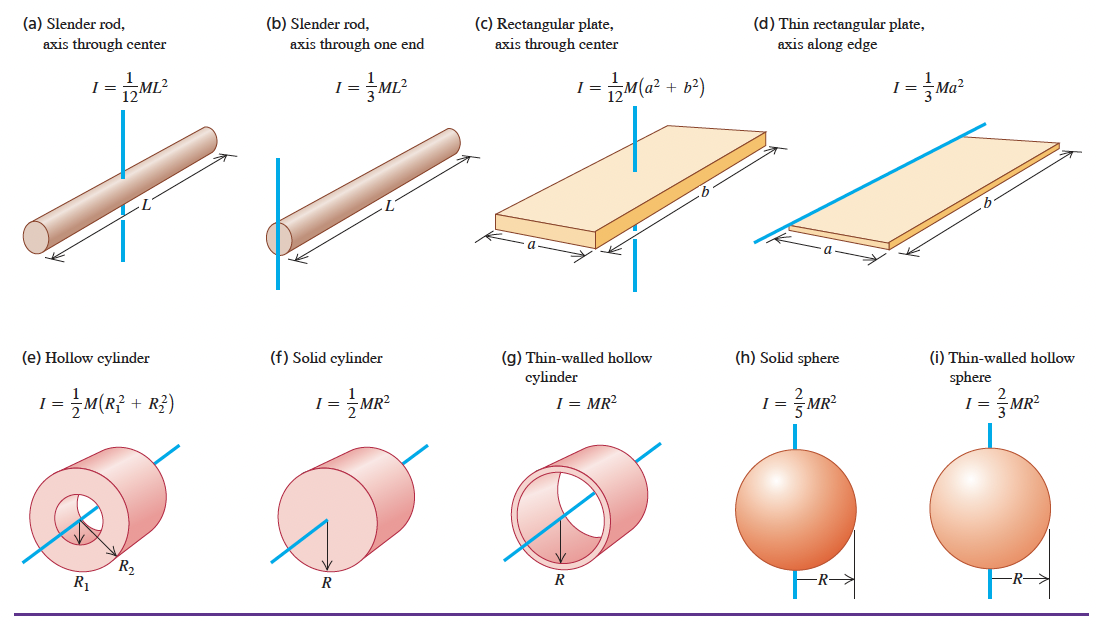
\includegraphics[width=0.8\linewidth]{../figures/F1.png}
  \label{fig:F1}
\end{figure}


\subsection{Parallel-akse-teoremet} \label{afs:parakstheo}
Parallel-akse-teoremet foreskriver at
\[ 
I_{P} = I_{\text{cm}} + Md^2
.\]
Hvor $M$ er massen af legemet, $I_{P}$ er inertimomentet for rotation gennem punktet $P$, $I_{\text{cm}}$ er inertimomentet for en akse gennem legemets massemidtpunkt, der er parallel med aksen gennem $P$ og $d$ er afstanden fra massemidtpunktet til punktet $P$.

    \newpage
    \section{Rotationsdynamik}

\begin{table}[ht]
\begin{tabular}{|l|l|l|}
\hline
\textbf{Givet}                           & \textbf{Ønsker at finde}      & \textbf{Relevante formler}   \\ \hline
Kraft, "arm" eller vinkel og afstand     & Kraftmomentets størrelse      & \ref{afs:strkramom}          \\ \hline
Kraft, arm                               & Kraftmomentvektoren           & \ref{afs:kramomvek}          \\ \hline
Inertimoment, vinkelacceleration         & Kraftmoment                   & \ref{afs:new2rig}            \\ \hline
\begin{tabular}[c]{@{}l@{}}Masse, hastighed af massemidtpunkt,\\ inertimoment, vinkelhastighed\end{tabular} &
  \begin{tabular}[c]{@{}l@{}}Kinetisk energi for legeme\\ med rotationel og translatorisk\\ bevægelse\end{tabular} &
  \ref{afs:erottrans} \\ \hline
Radius, vinkelhastighed (ingen glidning) & Hastighed                     & \ref{afs:ruluglid}           \\ \hline
Kraftmoment, start- og slutvinkel        & Arbejde udført af kraftmoment & \ref{afs:wortor}             \\ \hline
\begin{tabular}[c]{@{}l@{}}Konstant kraftmoment, start- og\\ slutvinkel\end{tabular} &
  Arbejde udført af kraftmoment &
  \ref{afs:wortorkon} \\ \hline
Inertimoment, vinkelhastighed            & Samlet arbejde                & \ref{afs:wortorvinhasinemom} \\ \hline
Kraftmoment, vinkelhastighed             & Effekt                        & \ref{afs:effkramom}          \\ \hline
Afstand, impuls                          & Impulsmoment                  & \ref{afs:impmomtanimp}       \\ \hline
Afstand, masse, hastighed                & Impulsmoment                  & \ref{afs:impmomtanimp}       \\ \hline
Inertimoment, vinkelhastighed            & Impulsmoment                  & \ref{afs:impmomvinhas}       \\ \hline
\end{tabular}
\end{table}

\subsection{Kraftmoment (10.1)}

\subsubsection{Størrelsen af kraftmomentet} \label{afs:strkramom}
Størrelsen på kraftmomentet $\tau$ forårsaget af kraften $\Vec{F}$ omkring punktet $O$ kan findes som
\[ 
\tau = Fl = rF \sin\phi = F_{\text{tan}} r
.\]
Hvor $F$ er størrelsen på $\Vec{F}$, $l$ er ``armen'' til $\Vec{F}$, $r$ er størrelsen på stedvektoren fra $O$ til $\Vec{F}$, $\phi$ er vinklen mellem $\Vec{r}$ og $\Vec{F}$ og $F_{\text{tan}}$ er den tangentielle komposant af $\Vec{F}$.


\subsubsection{Kraftmomentvektoren} \label{afs:kramomvek}
Kraftmomentvektoren $\Vec{\tau}$ forårsaget af $\Vec{F}$ omkring punktet $O$ kan findes som
\[ 
\Vec{\tau} = \Vec{r} \times \Vec{F}
.\]
Hvor $\Vec{r}$ er stedvektoren fra $O$ til $\Vec{F}$.


\subsection{Kraftmoment og vinkelacceleration for et rigidt legeme (10.2)}

\subsubsection{Newtons 2. lov et rigidt legeme} \label{afs:new2rig}
Givet inertimomentet $I$ og vinkelaccelerationen omkring $z$-aksen $\alpha_z$ kan det samlede kraftmoment omkring $z$-aksen $\sum\tau_z$ findes som
\[ 
\sum \tau_z = I \alpha_z
.\]

\subsection{Rotation for et rigidt legeme omkring en akse i bevægelse (10.3)}

\subsubsection{Kinetisk energi for et legeme med rotationel og translatorisk bevægelse} \label{afs:erottrans}
Givet massen af legemet $M$, massemidtpunktets hastighed $v_{\text{cm}}$, inertimomentet omkring omdrejningsaksen igennem massemidtpunktet $I_{\text{cm}}$ og vinkelhastigheden $\omega$ kan den samlede kinetiske energi $K$ findes som
\[ 
K = \frac{1}{2}Mv_{\text{cm}}^2 + \frac{1}{2}I_{\text{cm}}\omega^2
.\]


\subsubsection{Rulning uden glid (Eng: \textit{Rolling without slipping})} \label{afs:ruluglid}
Givet radiussen $R$ og vinkelhastigheden $\omega$ for et hjul kan massemidtpunktets hastighed $v_{\text{cm}}$ findes som 
\[ 
v_{\text{cm}} = R\omega
.\]


\subsection{Arbejde og effekt for roterende bevægelse (10.4)}

\subsubsection{Arbejdet udført af et kraftmoment} \label{afs:wortor}
Arbejdet $W$ udført af kraftmomentet $\tau_z$ kan findes som integralet af kraftmomentet ift. vinklen $\theta$ som
\[ 
W = \int_{\theta_1}^{\theta_2} \tau_z \, \mathrm{d}\theta
.\]
Hvor $\theta_1$ og $\theta_2$ er start- og slutvinklen


\subsubsection{Arbejdet udført af et konstant kraftmoment} \label{afs:wortorkon}
Holdes kraftmomentet $\tau_z$ konstant kan det vises at resultatet fra \ref{afs:wortor}: \nameref{afs:wortor} reduceres til
\[ 
W = \tau_z (\theta_2 - \theta_1) = \tau_z \Delta \theta
.\]


\subsubsection{Arbejdet udført af et kraftmoment givet vinkelhastighed og inertimoment} \label{afs:wortorvinhasinemom}
Givet et inertimoment $I$ og en start- og slutwinkelhastighed $\omega_1$ og $\omega_2$ kan det totale arbejde $W_{\text{tot}}$ udført af kraftmomentet findes som
\[ 
W_{\text{tot}} = \int_{\omega_1}^{\omega_2} I\omega_z \, \mathrm{d}\omega_z = \frac{1}{2}I \omega_2^2 - \frac{1}{2}I\omega_1^2
.\]


\subsubsection{Effekten af et kraftmoment} \label{afs:effkramom}
For et kraftmoment $\tau_z$ der virker omkring et legemes rotationsakse og vinkelhastigheden $\omega_z$ om selvsamme rotationsakse kan effekten $P$ forårsaget af kraftmomentet findes som
\[ 
P = \tau_z \omega_z
.\]

\subsection{Impulsmoment (10.5)}

\subsubsection{Impulsmomentet givet tangentiel impuls eller -hastighed} \label{afs:impmomtanimp}
Givet positionsvektoren $\Vec{r}$ og den tangentielle impuls $\Vec{p}$ eller den tangentielle hastighed $\Vec{v}$ kan impulsmomentet $\Vec{L}$ findes som
\[ 
\Vec{L} = \Vec{r} \times \Vec{p} = \Vec{r} \times m \Vec{v}
.\]

\subsubsection{Impulsmomentet givet vinkelhastighed} \label{afs:impmomvinhas}
Givet inertimomentet $I$ og vinkelhastigheden $\Vec{\omega}$ kan impulsmomentet $\Vec{L}$ findes som
\[ 
\Vec{L} = I \Vec{\omega}
.\]


\subsubsection{Sammenhæng mellem impulsmoment og kraftmoment}
Det gælder at
\[ 
\sum \Vec{\tau} = \frac{\mathrm{d}\Vec{L}}{\mathrm{d}t} 
.\]
Hvor $\sum \Vec{\tau}$ er summen af kraftmomenterne og $\frac{\mathrm{d}\Vec{L}}{\mathrm{d}t}$ er ændringen i impulsmoment over tid.


\subsection{Konservation af impulsmoment (10.6)}
Når summen af kraftmomenter der virker på et system er 0 og massen af systemet ikke ændrer sig (altså at systemet er lukket) så er det totale impulsmoment konserveret.

    \newpage
    \section{Ligevægt og elasticitet}

\begin{table}[ht]
\begin{tabular}{|l|l|l|}
\hline
\textbf{Givet}       & \textbf{Ønsker at finde} & \textbf{Relevante formler} \\ \hline
Kraft, areal         & Spænding                 & \ref{afs:stress}           \\ \hline
Start- og slutlængde & Tøjning                  & \ref{afs:strain}           \\ \hline
Spænding, tøjning    & Youngs modul             & \ref{afs:young}            \\ \hline
Spænding, tøjning    & Kompressibilitetsmodul   & \ref{afs:kompmod}          \\ \hline
Spænding, tøjning    & Forskydningsmodul        & \ref{afs:formod}           \\ \hline
\end{tabular}
\end{table}

\subsection{Ligevægtsbetingelser (11.1)}

\subsubsection{Summen af kræfter for ligevægt (Den første ligevægtsbetingelse)}
For et objekt i ligevægt gælder at
\[ 
\sum \Vec{F} = 0
.\]
Hvor $\sum \Vec{F}$ er summen af alle eksterne kræfter på objektet.

\subsubsection{Summen af kraftmomenter for ligevægt (Den anden ligevægtsbetingelse)}
For et objekt i ligevægt gælder at
\[ 
\sum \Vec{\tau} = 0
.\]
Hvor $\sum \Vec{\tau}$ er summen af alle eksterne kraftmomenter på objektet.


\subsection{Løsningsmetode for ligevægtsproblemer for rigide legemer (11.3)}
For at løse et ligevægtsproblem for et rigidt legeme kræver det typisk at man opskriver ligevægtsbetingelserne
\[ 
\sum F_x = 0, \qquad \sum F_y = 0, \qquad \sum \tau_z = 0
\]
og løser de tre ligninger med tre ubekendte. Det kan være en hjælp at kigge i \ref{sec:cm}: \nameref{sec:cm}.


\subsection{Spænding, tøjning og elasticitetsmodul (11.4)}

\subsubsection{Hookes lov} \label{afs:hooke}
Hookes lov foreskriver at
\[ 
Y = \frac{\sigma}{\epsilon}
.\]
Dette gælder såfremt spændingen $\sigma$ og den resulterende tøjning $\epsilon$ på objektet er tilpas små (er under proportionalitetsgrænsen).

\subsubsection{Spænding} \label{afs:stress}
Trækspændingen $\sigma_{\text{træk}}$ er givet som
\[ 
\sigma_{\text{træk}} = \frac{F_{\perp}}{A}
.\]
Hvor $F_{\perp}$ er kraften vinkelret på overfladen med areal $A$.


\subsubsection{Tøjning} \label{afs:strain}
Træktøjningen $\epsilon_{\text{træk}}$ er givet som
\[ 
\epsilon_{\text{træk}} = \frac{l - l_0}{l_0} = \frac{\Delta l}{l_0}
.\]
Hvor $l$ og $l_0$ er hhv. slut- og startlængden.


\subsubsection{Youngs modul} \label{afs:young}
Ved at indsætte udtrykkene fra \ref{afs:stress}: \nameref{afs:stress} og \ref{afs:strain}: \nameref{afs:strain} ind i udtrykket fra \ref{afs:hooke}: \nameref{afs:hooke} fås at
\[
  Y = \frac{\sigma}{\epsilon} = \frac{F_{\perp} / A}{\Delta l / l_0} = \frac{F_{\perp}}{A} \frac{l_0}{\Delta l}
.\]
Hvor $Y$ er Younds modul, $F_{\perp}$ er den vinkelrette kraft, $A$ er tværsnitsarealet af objektet, $l_0$ er startlængden og $\Delta l$ er forlængelsen.


\subsubsection{Tabel over elasticitetsmoduler}
\begin{table}[ht]
\centering
\begin{tabular}{lccc}
\hline
\textbf{Materiale} &
  \multicolumn{1}{l}{\textbf{\begin{tabular}[c]{@{}l@{}}Youngs modul,\\ $Y$ (\unit{Pa})\end{tabular}}} &
  \multicolumn{1}{l}{\textbf{\begin{tabular}[c]{@{}l@{}}Kompressibilitetsmodul,\\ $B$ (\unit{Pa})\end{tabular}}} &
  \multicolumn{1}{l}{\textbf{\begin{tabular}[c]{@{}l@{}}Forskydningsmodul,\\ $S$ (\unit{Pa})\end{tabular}}} \\ \hline
Aluminium & \num{7,0e10}   & \num{7,5e10} & \num{2,5e10}    \\
Messing   & \num{9,0e10}   & \num{6,0e10} & \num{3,5e10}    \\
Kobber    & \num{11e10}    & \num{14e10}  & \num{4,4e10}    \\
Jern      & \num{21e10}    & \num{16e10}  & \num{7,7e10}    \\
Bly       & \num{1,6e10}   & \num{4,1e10} & \num{0,6e10}    \\
Nikkel    & \num{21e10}    & \num{17e10}  & \num{7,8e10}    \\
Silikone  & \num{0,001e10} & \num{0,2e10} & \num{0,0002e10} \\
Stål      & \num{20e10}    & \num{16e10}  & \num{7,5e10}    \\
Ledbånd   & \num{0,12e10}  & –            & –               \\ \hline
\end{tabular}
\end{table}


\subsubsection{Kompressibilitetsmodul} \label{afs:kompmod}
Kompressibilitetsmodulet $B$ er givet som
\[ 
B = \frac{\sigma_{\text{tryk}}}{\epsilon_{\text{tryk}}} = - \frac{\Delta p}{\Delta V / V_0}
.\]
Hvor $\Delta p$ er ændringen i trykket, der forårsager kompressionen, $\Delta V$ er ændringen i volumen og $V_0$ er initialvolumenet


\subsubsection{Forskydningsmodul} \label{afs:formod}
\begin{figure} [ht]
  \centering
  \caption{Figur til forklaring af forskydningsmodulet}
  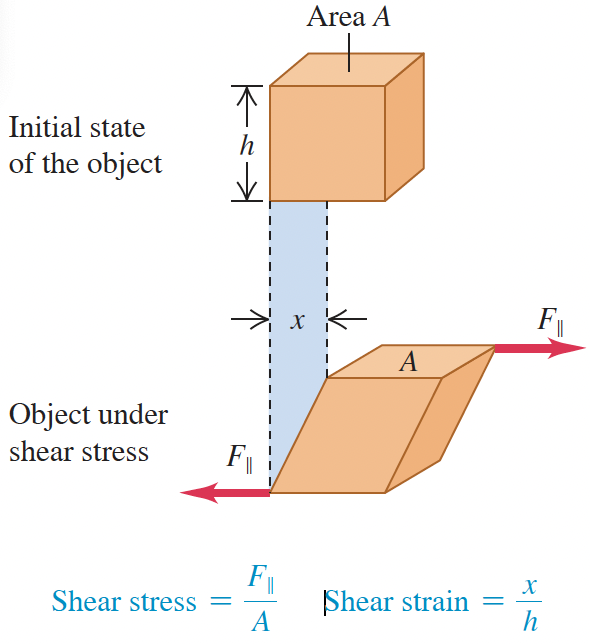
\includegraphics[width=0.2\linewidth]{../figures/F2.png}
  \label{fig:F2}
\end{figure}

Forskydningsmodulet $S$ kan findes som
\[ 
S = \frac{\sigma_{\text{forskydning}}}{\epsilon_{\text{forskydning}}} = \frac{F_{\parallel} / A}{x / h} = \frac{F_{\parallel}}{A} \frac{h}{x}
.\]
Hvor $F_{\parallel}$ er kraften der påføres parallelt med ovjektets overflade, $A$ er arealet som kraften arbejder over, $x$ er deformationen og $h$ er den tværgående afstand (se evt. \textbf{\autoref{fig:F2}} fra bogens side 350).


\subsection{Perturbationsteoretisk ligevægt}
Fra perturbationsteori har vi at et system i ligevægt er stabilt (en lille ændring i systemet ødelægger ikke ligevægten) såfremt
\[ 
\frac{\mathrm{d}U^2}{\mathrm{d}^2x} > 0
,\]
Hvor $U$ er potentiel energi og $x$ er position. Dette resultat gælder eftersom enhver lille forskydning af massen dx i dette tilfælde medfører en restaurerende kraft og vice versa.
 
    \newpage
    \section{Fluidmekanik}

\begin{table}[ht]
\begin{tabular}{|l|l|l|}
\hline
\textbf{Givet}                   & \textbf{Ønsker at finde}         & \textbf{Relevante formler} \\ \hline
Masse, volumen                   & Densitet                         & \ref{afs:dens}             \\ \hline
Kraft, areal                     & Tryk                             & \ref{afs:trykdef}          \\ \hline
Densitet, højdeforskel           & Trykforskel                      & \ref{afs:trykfor}          \\ \hline
Densitet, dybde                  & Tryk til dybde                   & \ref{afs:trykdyb}          \\ \hline
Densitet, volumen                & Opdriftskraft                    & \ref{afs:ark}              \\ \hline
Areal, strømningshastighed       & Volumenstrømningshastighed       & \ref{afs:volstr}           \\ \hline
Tryk, densitet, dybde, hastighed & Tryk, densitet, dybde, hastighed & \ref{afs:bern}             \\ \hline
\end{tabular}
\end{table}

\subsection{Densitet og tryk (12.1-12.2)}

\subsubsection{Densiteten af et homogent legeme} \label{afs:dens}
Givet et homogent legemes masse $m$ og dets volumen $V$ kan densitet $\rho$ findes som
\[ 
\rho = \frac{m}{V}
.\]


\subsubsection{Definition af tryk i en væske} \label{afs:trykdef}
Trykket $p$ i en væske er defineret som
\[ 
p = \frac{\mathrm{d}F_{\perp}}{\mathrm{d}A} 
.\]
Hvor $\mathrm{d}F_{\perp}$ er normalkraften udøvet af en væske på en lille overflade med overfladeareal $\mathrm{d}A$.


\subsubsection{Trykforskel mellem to punkter i en væske med uniform densitet} \label{afs:trykfor}
Trykforskellen $p_2 - p_1$ mellem to punkter i en væske med uniform densitet er givet ved
\[ 
p_2 - p_1 = -\rho g(y_2 - y_1)
.\]
Hvor $\rho$ er den uniforme densitet, $g$ er tyngdeaccelerationen og $y_2$ og $y_1$ er højden til to forskellige punkter. 


\subsubsection{Trykket til en given dybde i en væske med uniform densitet} \label{afs:trykdyb}
Givet et initialtryk $p_0$, en densitet $\rho$ og dybden $h$ kan trykket $p$ findes som
\[ 
p = p_0 + \rho gh
.\]


\subsubsection{Pascals lov}
Pascals lov siger at: ``Tryk, der påføres en indelukket væske, overføres uformindsket til alle dele af væsken og væggene i det beholdende kar.''


\subsubsection{Absolut tryk og overtryk (manometertryk)}
Det totale tryk (inkl. atmosfærisk tryk) kaldes normalt for absolut tryk og \textit{overtrykket} ift. atmosfærisk tryk (altså det totale tryk minus det absolutte tryk) kaldes normalt overtrykket eller manometertrykket.


\subsection{Opdrift (12.3)}

\subsubsection{Arkimedes princip}
Arkimedes princip siger at: ``Når en genstand er helt eller delvist nedsænket i en væske, udøver væsken en opadrettet kraft på genstanden, der er lig med vægten af den væske, som genstanden fortrænger.''


\subsubsection{Matematisk formulering af Arkimedes princip} \label{afs:ark}
Givet densiteten af en uniform væske $\rho$, volumenet af den fortrængte væske $V$ og tyngdeaccelerationen $g$ kan opdriftskraften $F_{b}$ findes som
\[
F_b = \rho Vg
.\]

\subsection{Væskestrømning (Eng: \textit{Fluid Flow}) (12.4)}

\subsubsection{Ideele væsker}
En \textit{ideel} væske er en matematisk model der simplificerer fluidmekanik. Det antages at en ideel væske er
\begin{itemize}
  \item \textbf{Inkompressibel}: Altså at væskens densitet ikke kan ændres
  \item \textbf{Inviskos}: Altså at væsken ingen indre friktion har
\end{itemize}
De fleste væsker kan under normale omstændigheder antages at være inkompressible -- det samme gør sig gældende for gasser, så længe trykforskellene ikke er for store. Inviskositet er et rimeligt krav for letflydende væsker og gasser såfremt de andre kræfter der virker på væsken eller gassen er væsentligt større end den interne friktion ville være.


\subsubsection{Kontinuitetsligningen} \label{afs:kontin}
Kontinuitetsligningen for en inkompressibel væske er
\[ 
A_1v_1 = A_2v_2
.\]
Hvor $v_1$ og $v_2$ er strømningshastigheden to forskellige steder og $A_1$ og $A_2$ er tværsnitsarealerne de samme to steder. 


\subsubsection{Volumenstrømningshastighed} \label{afs:volstr}
Produktet $Av$ fra \ref{afs:kontin}: \nameref{afs:kontin} er lig volumenstrømningshastigheden $\frac{\mathrm{d}V}{\mathrm{d}t}$. Altså
\[ 
\frac{\mathrm{d}V}{\mathrm{d}t} = Av
.\]


\subsection{Bernoullis ligning (12.5)}

\subsubsection{Bernoullis ligning} \label{afs:bern}
Bernoullis ligning er
\[ 
  p + \rho gy + \frac{1}{2}\rho v^2 = \text{const.}
.\]
Hvor $p$ er trykket, $\rho$ er væskens densitet, $g$ er tyngdeaccelerationen, $y$ er elevationen og $v$ er hastigheden. \textbf{Bemærk}: Bernoullis ligning gælder kun for idelle væsker med stationær strømning. Denne kan også skrives som
\[ 
p_1 + \rho g y_1 + \frac{1}{2} \rho v_1^2 = p_2 + \rho g y_2 + \frac{1}{2} \rho v_2^2
.\]


    \newpage
    \section{Gravitation}

\begin{table}[ht]
\begin{tabular}{|l|l|l|}
\hline
\textbf{Givet}                   & \textbf{Ønsker at finde}           & \textbf{Relevante formler} \\ \hline
To masser, afstand               & Tyngdekraft                        & \ref{afs:newtyn}           \\ \hline
To masser, afstand               & Tyngde                             & \ref{afs:tyngde}           \\ \hline
Masse af objekt, radius af objekt & Tyngdeacceleration ved overflade & \ref{afs:tynacc} \\ \hline
To masser, to afstande           & Tyngdekraftens arbejde             & \ref{afs:tynarb}           \\ \hline
To masser, afstand               & Potentiel energi for tyngdekraften & \ref{afs:tynpot}           \\ \hline
Masse, kredsløbsradius           & Hastighed af sattelit              & \ref{afs:hassat}           \\ \hline
Kredsløbsradius, omløbshastighed & Periode for sattelit               & \ref{afs:persat}           \\ \hline
\end{tabular}
\end{table}

\subsection{Newtons tyngdelov (13.1)}

\subsubsection{Newtons tyngdelov}
Newtons tyngdelov siger at: ``Enhver partikel i universet tiltrækker enhver anden partikel med en kraft, der er direkte proportional med produktet af partikernes masser og omvendt proportional med kvadratet af afstanden mellem dem.''

\subsubsection{Matematisk formulering af Newtons tyngdelov} \label{afs:newtyn}
Matematisk kan Newtons tyngdelov formuleres som
\[ 
F_g = \frac{Gm_1m_2}{r^2}
.\]
Hvor $F_g$ er tyngdekraften, $G \approx \qty{6,67408e-11}{N.m^2.kg^{-2}} $ er gravitationskonstanten, $m_1$ og $m_2$ er masserne af de to legemer som påvirker hinanden gravitationelt og $r$ er afstanden mellem de to legemer.


\subsection{Tyngde (Eng: \textit{Weight}) (13.2)}

\subsubsection{Tyngden af et objekt ved jordens overflade} \label{afs:tyngde}
Tyngden $w$ af et objekt ved jordens overflade er lig tyngdekraften fra jorden på objektet. Altså
\[ 
w = F_g = \frac{Gm_Em}{R_E^2}
.\]
Hvor $m_E$ er jordens masse, $R_E$ er jordens radius og $m$ er massen af objektet, hvis tyngde man ønsker at finde.


\subsubsection{Tyngdeaccelerationen} \label{afs:tynacc}
Tyngdeaccelerationen ved jordens overflade $g$ kan findes som
\[ 
g = \frac{Gm_E}{R_E^2}
.\]
Hvor $m_E$ er jordens masse og $R_E$ er jordens radius. 


\subsection{Potentiel energi i et tyngdefelt (13.3)}

\subsubsection{Tyngdekraftens arbejde} \label{afs:tynarb}
Tyngdekraftens arbejde $W_{\text{grav}}$ kan findes som
\[ 
W_{\text{grav}} = -GMm \int_{r_1}^{r_2} \frac{\mathrm{d}r}{r^2} = \frac{GMm}{r_2} - \frac{GMm}{r_1} 
.\]
Hvor $M$ og $m$ er masserne af de to objekter tyngdekraften yder et arbejde på og $r_1$ og $r_2$ er hhv. start- og slutafstanden mellem de to masser.


\subsubsection{Potentiel energi i et tyngdefelt} \label{afs:tynpot}
Den potentielle energi i et tyngdefelt $U$ på et objekt med masse $m$ kan findes som
\[ 
U = - \frac{GMm}{r}
.\]
Hvor $M$ er massen af objektet som påvirker massen $m$ og $r$ er den indbyrdes afstand mellem massemidtpunktet af massen $M$ og massemidtpunktet af massen $m$.


\subsection{Satellitter i cirkulær bevægelse (13.4)}

\subsubsection{Hastigheden af en satellit i et cirkulært kredsløb} \label{afs:hassat}
For en sattelit i et cirkulært kredsløb om en masse $M$ med en kredsløbsradius på $r$ kan hastigheden af satellitten $v$ findes som
\[ 
v = \sqrt{\frac{GM}{r}}
.\]

\subsubsection{Perioden for en satellit i et cirkulært kredsløb} \label{afs:persat}
For en sattelit med hastighed $v$ i en cirkulær bane med radius $r$ omkring et legeme med masse $M$ kan perioden $T$ findes som
\[ 
T = \frac{2\pi r}{v} = 2\pi r \sqrt{\frac{r}{GM}} = \frac{2\pi r^{\frac{3}{2}}}{\sqrt{GM}}
.\]


\subsection{Keplers love og planeters bevægelse (13.5)}

\subsubsection{Keplers love}
Keplers love lyder
\begin{enumerate}
  \item Alle planeter bevæger sig i elliptiske baner omkring Solen, hvor Solen befinder sig i det ene brændpunkt.
  \item En linje trukket fra en planet til Solen overstryger lige store arealer på lige lange tidsrum.
  \item Kvadratet af en planets omløbstid er proportionalt med kuben af dens middelafstand fra Solen.
\end{enumerate}


\subsubsection{Matematisk formulering af Keplers 2. lov}
Keplers 2. lov kan skrives som
\[ 
\frac{\mathrm{d}A}{\mathrm{d}t} = \frac{1}{2}r^2 \frac{\mathrm{d}\theta}{\mathrm{d}t} 
.\]
Hvor $r$ er radiussen af planetens bane og $\mathrm{d}\theta$ og $\mathrm{d}A$ er hhv. vinklen der tilbagelægges og arealet der overstryges i det lille tidsinterval $\mathrm{d}t$.

\subsubsection{Matematisk formulering af Keplers 3. lov}
Keplers 3. lov kan skrives som
\[ 
T = \frac{2\pi a^{\frac{3}{2}}}{\sqrt{Gm_s}}
.\]
Hvor $T$ er perioden, $a$ er planetens middelafstand fra en sol med massen $m_s$. 



\subsection{Sorte huller (13.8)}

\subsubsection{Swarzschild-radiussen af et sort hul}
Radiussen som en masse $M$ maksimalt må have for at opføre sig som et sort hul betegnes massens Schwarz\-schild-radius $R_s$ og kan findes som
\[ 
R_s = \frac{2GM}{c^2}
.\]
Hvor $c$ er lysets hastighed i et vakuum.

    \newpage
    \section{Periodisk bevægelse}

\begin{table}[ht]
\begin{tabular}{|l|l|l|}
\hline
\textbf{Givet} &
  \textbf{Ønsker at finde} &
  \textbf{Relevante formler} \\ \hline
Periode &
  Frekvens &
  \ref{afs:frekper} \\ \hline
Periode eller frekvens &
  Vinkelfrekvens &
  \ref{afs:vinfrek} \\ \hline
Fjederkonstant, forskydning &
  Kraft i SHM &
  \ref{afs:SHMkra} \\ \hline
Fjederkonstant, masse, forskydning &
  Acceleration i SHM &
  \ref{afs:SHMacc} \\ \hline
Fjederkonstant, masse &
  Vinkelfrekvens i SHM &
  \ref{afs:SHMvinfrek} \\ \hline
Vinkelfrekvens &
  Frekvens i SHM &
  \ref{afs:SHMfrek} \\ \hline
Fjederkonstant, masse &
  Frekvens i SHM &
  \ref{afs:SHMfrek} \\ \hline
Frekvens &
  Periode i SHM &
  \ref{afs:SHMper} \\ \hline
\begin{tabular}[c]{@{}l@{}}Amplitude, vinkelfrekvens, tid, \\ faseforskydning\end{tabular} &
  Position i SHM &
  \ref{afs:SHMpos} \\ \hline
\begin{tabular}[c]{@{}l@{}}Masse, hastighed, fjederkonstant,\\  forskydning, amplitude\end{tabular} &
  Mekanisk energi i SHM &
  \ref{afs:emekSHM} \\ \hline
Kraftkonstant og mase &
  \begin{tabular}[c]{@{}l@{}}Vinkelfrekvens for simpelt\\ pendul\end{tabular} &
  \ref{afs:vinfrekspen} \\ \hline
Længde &
  \begin{tabular}[c]{@{}l@{}}Vinkelfrekvens for simpelt\\ pendul\end{tabular} &
  \ref{afs:vinfrekspen} \\ \hline
Vinkelfrekvens eller længde &
  Periode for simpelt pendul &
  \ref{afs:perspen} \\ \hline
Masse, længde, inertimoment &
  \begin{tabular}[c]{@{}l@{}}Vinkelfrekvens for fysisk\\ pendul\end{tabular} &
  \ref{afs:vinfrekfpen} \\ \hline
Inertimoment, masse, længde &
  Periode for fysisk pendul &
  \ref{afs:perfpen} \\ \hline
\begin{tabular}[c]{@{}l@{}}Amplitude, dæmpningskonstant, \\ masse, vinkelfrekvens, tid, \\ faseforskydning\end{tabular} &
  \begin{tabular}[c]{@{}l@{}}Forskydning i dæmpet\\ oscillation\end{tabular} &
  \ref{afs:foroscdæmp} \\ \hline
Kraftkonstant, masse, dæmpningskonstant &
  \begin{tabular}[c]{@{}l@{}}Vinkelfrekvens i dæmpet\\ oscillation\end{tabular} &
  \ref{afs:vinfrekoscdæmp} \\ \hline
\begin{tabular}[c]{@{}l@{}}Størrelsen af drivkraften, kraftkonstant,\\ masse, drivende vinkelfrekens,\\ dæmpningskonstant\end{tabular} &
  \begin{tabular}[c]{@{}l@{}}Amplitude af tvungen\\ oscillation\end{tabular} &
  \ref{afs:amptvu} \\ \hline
\begin{tabular}[c]{@{}l@{}}Initialamplitude, dæmpningskonstand,\\ masse, tid\end{tabular} &
  \begin{tabular}[c]{@{}l@{}}Amplitude til tid \\af dæmpet oscillation\end{tabular} &
  \ref{afs:ampdæmtid} \\ \hline
\begin{tabular}[c]{@{}l@{}}Inertimoment, kraft,\\ kraftarm\end{tabular} &
  \begin{tabular}[c]{@{}l@{}}Bevægelsesligning for pendul\end{tabular} &
  \ref{afs:bevpen} \\ \hline
\end{tabular}
\end{table}


\subsection{Beskrivelse af oscillationer (14.1)}

\subsubsection{Forholdet mellem frekvens og periode} \label{afs:frekper}
Det gælder at frekvensen af en oscillation $f$ og perioden af selvsamme $T$ er inverst proportionelle. Altså at
\[ 
f = \frac{1}{T} \iff T = \frac{1}{f}
.\]

\subsubsection{Vinkelfrekvens og periode eller frekvens} \label{afs:vinfrek}
Vinkelfrekvensen $\omega$ forholder sig til frekvensen $f$ og perioden $T$ som
\[ 
\omega = 2\pi f = \frac{2\pi}{T}
.\]


\subsection{Simpel harmonisk bevægelse (SHM) (14.2)}

\subsubsection{Kraften for SHM (Fjederkraften)} \label{afs:SHMkra}
For ideelle fjedre (dvs. dem der overholder \ref{afs:hooke}: \nameref{afs:hooke}) gælder at 
\[ 
F_x = -kx
.\]
Hvor $F_x$ er den restaurerende kraft udøvet af fjederen, $k$ er fjederkonstanten og $x$ er forskydningen. 

\subsubsection{Acceleration for SHM} \label{afs:SHMacc}
Accelerationen $a_x$ for SHM kan findes som
\[ 
a_x = \frac{\mathrm{d}^2x}{\mathrm{d}t^2} = - \frac{k}{m}x
.\]
Hvor $x$ er forskydningen, $k$ er fjederkonstanten og $m$ er massen af objektet der laver SHM. 


\subsubsection{Vinkelfrekvens for SHM} \label{afs:SHMvinfrek}
Vinkelfrekvensen $\omega$ for et objekt der undergår $SHM$ kan findes som
\[ 
\omega = \sqrt{\frac{k}{m}}
.\]
Hvor $k$ er fjederkonstanten og $m$ er massen af objektet.


\subsubsection{Frekvens for SHM} \label{afs:SHMfrek}
Frekvensen $f$ for et objekt der undergår SHM kan findes som
\[ 
f = \frac{\omega}{2\pi} = \frac{1}{2\pi}\sqrt{\frac{k}{m}}
.\]
Hvor $\omega$ er vinkelfrekvensen, $k$ er fjederkonstanten og $m$ er massen af objektet.


\subsubsection{Perioden for SHM} \label{afs:SHMper}
Perioden $T$ for et objekt der undergår SHM kan findes som
\[ 
T = \frac{1}{f} = \frac{2\pi}{\omega} = 2\pi \sqrt{\frac{m}{k}}
.\]
Hvor $f$ er frekvensen, $\omega$ er vinkelhastigheden, $m$ er massen af objektet og $k$ er fjederkonstanten.


\subsubsection{Position som funktion af tid for SHM} \label{afs:SHMpos}
Givet en amlitude $A$, en vinkelfrekvens $\omega$ og en faseforskydning $\phi$ kan forskydningen af et objekt $x$ der undergår SHM til tiden $t$ findes som
\[ 
x = A \cos (\omega t + \phi)
.\]

\subsection{Energi i SHM (14.3)}

\subsubsection{Mekanisk energi for SHM} \label{afs:emekSHM}
Den totale mekaniske energi $E$ kan for et objekt der undergår SHM findes som
\[ 
E = \frac{1}{2}mv_x^2 + \frac{1}{2}kx^2 = \frac{1}{2}kA^2 = \text{const.}
.\]
Hvor $m$ er massen af objektet, $v_x$ er hastigheden, $k$ er fjederkonstanten, $x$ er forskydningen og $A$ er amplituden. 


\subsection{Det simple pendul (14.5)}

\subsubsection{Vinkelfrekvensen for et simpelt pendul} \label{afs:vinfrekspen}
For et simpelt (matematisk) pendul med tilpas lav amplitude kan vinkelfrekvensen $\omega$ findes som
\[ 
\omega = \sqrt{\frac{k}{m}} = \sqrt{\frac{g}{L}}
.\]
Hvor $k$ er pendulets kraftkonstant ($k = \frac{mg}{L}$), $m$ er pendulets masse og $L$ er pendulets længde.


\subsubsection{Frekvens af et simpelt pendul} \label{afs:frekspen}
For et simpelt pendul med tilpas lav amplitude kan frekvensen $f$ findes som
\[ 
f = \frac{\omega}{2\pi} = \frac{1}{2\pi} \sqrt{\frac{g}{L}}
.\]
Hvor $\omega$ er vinkelfrekvensen og $L$ er pendulets længde.


\subsubsection{Periode for et simpelt pendul} \label{afs:perspen}
For et simpelt pendul med tilpas lav amplitude kan perioden $T$ findes som
\[ 
T = \frac{1}{f} = \frac{2\pi}{\omega} = 2\pi \sqrt{\frac{L}{g}}
.\]
Hvor $f$ er pendulets frekvens, $\omega$ er dets vinkelfrekvens og $L$ er dets længde.



\subsection{Det fysiske pendul (14.6)}

\subsubsection{Bevægelsesligningen for et pendul} \label{afs:bevpen}
Bevægelsesligningen for et pendul er
\[ 
I \frac{\mathrm{d}^2 \theta}{\mathrm{d}t^2} = - F\cdot r \theta 
.\]
Hvor $I$ er pendulets inertimoment, $F$ er kraften og $r$ er armen.


\subsubsection{Vinkelfrekvens for et fysisk pendul} \label{afs:vinfrekfpen}
Vinkelfrekvensen $\omega$ for et fysisk pendul med tilpas lav amplitude kan findes som
\[ 
\omega = \sqrt{\frac{mgd}{I}}
.\]
Hvor $m$ er pendulets masse, $d$ er afstanden fra rotationsaksen tilpendulets massemidtpunkt og $I$ er dets inertimoment.


\subsubsection{Perioden for et fysisk pendul} \label{afs:perfpen}
Perioden $T$ for et fysisk pendul med tilpas lav amplitude kan findes som
\[ 
  T = 2\pi\sqrt{\frac{I}{mgd}}
.\]
Hvor $m$ er pendulets masse, $d$ er afstanden fra rotationsaksen tilpendulets massemidtpunkt og $I$ er dets inertimoment.

\subsection{Dæmpede oscillationer (14.7)}

\subsubsection{Forskydningen af oscillator med dæmpning} \label{afs:foroscdæmp}
Givet en dæmpet oscillator med relativt lav dæmpningsgrad kan forskydningen $x$ som funktion af tiden $t$ findes som
\[ 
x(t) = Ae^{-\left( \frac{b}{2m} \right)t} \cos(\omega' t + \phi)
.\]
Hvor $A$ er den initiale amplitude, $b$ er en dæmpningskonstant, $m$ er massen af oscillatoren, $\omega'$ er vinkelfrekvensen af den dæmpede oscillation og $\phi$ er faseforskydningen


\subsubsection{Vinkelfrekvens af en dæmpet oscillation} \label{afs:vinfrekoscdæmp}
Vinkelfrekvensen af en dæmpet oscillation $\omega'$ kan findes som
\[ 
\omega' = \sqrt{\frac{k}{m}- \frac{b^2}{4m^2}}
.\]
Hvor $k$ er kraftkonstanten for den restaurerende kraft, $m$ er massen og $b$ er en dæmpningskonstant.


\subsubsection{Amplitude af dæmpet oscillation} \label{afs:ampdæmtid}
Givet en initialamplitude $A_1$, en dæmpningskonstant $b$ og en masse $m$ kan amplituden $A_2$ til tiden $t$ findes som
\[ 
A_2 = A_1 e^{-\frac{b}{2m}t}
.\]


\subsection{Tvungne oscillationer og resonans (14.8)}
En dæmpet oscillator vil over tid stoppe med at bevæge sig. Dette kan forhindres ved at tilføje en periodisk kraft (tænk at du skubber din ven på en gynge 1 gang pr. cyklus), denne kraft kaldes \textit{drivkraften}.

\subsubsection{Amplitude af tvungen oscillation} \label{afs:amptvu}
Amplituden af en tvungen oscillation $A$ kan findes som
\[ 
A = \frac{F_{\text{max}}}{\sqrt{\left( k - m\omega_d^2 \right)^2 + b^2\omega_d^2}}
.\]
Hvor $F_{\text{max}}$ er den største størrelse drivkraften antager, $k$ er kraftkonstanten af den restaurerende kraft, $m$ er massen, $\omega_d$ er den drivende vinkelfrekvens og $b$ er en dæmpningskonstant.

    \newpage
    \section{Mekaniske bølger}

\begin{table}[ht]
\begin{tabular}{|l|l|l|}
\hline
\textbf{Givet} &
  \textbf{Ønsker at finde} &
  \textbf{Relevante formler} \\ \hline
Bølgelænde, frekvens &
  Bølgehastighed &
  \ref{afs:bølhas} \\ \hline
\begin{tabular}[c]{@{}l@{}}Amplitude, vinkelhastighed, position, \\ bølgehastighed, tid\end{tabular} &
  Bølgefunktion &
  \ref{afs:bølfun} \\ \hline
\begin{tabular}[c]{@{}l@{}}Amplitude, position, bølgelængde, tid, \\ periode\end{tabular} &
  Bølgefunktion &
  \ref{afs:bølfun2} \\ \hline
\begin{tabular}[c]{@{}l@{}}Ampltide, bølgetal, position,\\ vinkelfrekvens, tid\end{tabular} &
  Bølgefunktion &
  \ref{afs:bølfun3} \\ \hline
Spænding, masse pr. længde &
  \begin{tabular}[c]{@{}l@{}}Bølgehastighed af trans-\\ versalbølge på en snor\end{tabular} &
  \ref{afs:hastra} \\ \hline
\begin{tabular}[c]{@{}l@{}}Masse pr. længde, spænding, \\ vinkelfrekvens, amplitude\end{tabular} &
  \begin{tabular}[c]{@{}l@{}}Gennemsnitseffekten for\\ sinusoidal bølge på snor\end{tabular} &
  \ref{afs:gnseffbølsno} \\ \hline
Intensitet og to afstande &
  Intensitet til anden afstand &
  \ref{afs:omvkvalov} \\ \hline
\begin{tabular}[c]{@{}l@{}}Ampltiude af stående bølge, bølgetal,\\ position, vinkelfrekvens, tid\end{tabular} &
  \begin{tabular}[c]{@{}l@{}}Bølgefunktion for stående\\ bølge\end{tabular} &
  \ref{afs:bølfunstå} \\ \hline
Bølgehastighed, længde på snor &
  Normalmoder for en snor &
  \ref{afs:normod} \\ \hline
Bølgehastighed, snorens længde &
  Fundamentalfrekvens &
  \ref{afs:funfrek} \\ \hline
Spænding, masse pr. længde &
  Fundamentalfrekvens &
  \ref{afs:funfrek} \\ \hline
\end{tabular}
\end{table}

\subsection{Periodiske bølger og matematiske beskrivelser heraf (15.2-15.3)}

\subsubsection{Bølgehastighed for periodiske bølger} \label{afs:bølhas}
Givet en periodisk bølges bølgelængde $\lambda$ og dens frekvens $f$ kan bølgehastigheden $v$ findes som
\[ 
v = \lambda f
.\]


\subsubsection{Bølgefunktion for en bølge givet vinkel- og bølgehastighed} \label{afs:bølfun}
Bølgefunktionen for en sinusoidal bølge i $+x$-retningen er givet ved
\[ 
y(x,t) = A \cos \left( \omega \left( \frac{x}{v} - t \right) \right)
.\]
Hvor $A$ er amplituden, $\omega$ er vinkelfrekvensen, $x$ er positionen, $v$ er bølgehastigheden og $t$ er tiden.


\subsubsection{Bølgefunktion for en bølge givet bølgelængde og periode} \label{afs:bølfun2}
Bølgefunktionen fra ovenfor kan også skrives som
\[ 
y(x,t) = A \cos \left( 2\pi \left( \frac{x}{\lambda} - \frac{t}{T} \right) \right)
.\]
Hvor $A$ er amplituden, $x$ er positionen, $\lambda$ er bølgelængden, $t$ er tiden og $T$ er perioden.


\subsubsection{Bølgefunktion givet bølgetal og vinkelhastighed} \label{afs:bølfun3}
Bølgefunktionen fra ovenfor kan også skrives som
\[ 
y(x,t) = A \cos (kx - \omega t)
.\]
Hvor $A$ er amplituden, $k$ er bølgetallet ($k = \frac{2\pi}{\lambda}$), $x$ er positionen, $\omega$ er vinkelfrekvensen og $t$ er tiden.


\subsubsection{Bølgeligningen}
Bølgeligningen er
\[ 
\frac{\partial^2 y(x,t)}{\partial x^2} = \frac{1}{v^2} \frac{\partial^2 y(x,t)}{\partial t^2}
.\]
Hvor $\frac{\partial^2 y(x,t)}{\partial x^2}$ er den anden partielt afledede med hensyn til $x$, $v$ er bølgehastigheden of $\frac{\partial^2 y(x,t)}{\partial t^2}$ er den anden partielt afledede med hensyn til $t$.


\subsection{Hastigheden af en transversal bølge (15.4)}

\subsubsection{Hastigheden af en transversal bølge på en snor} \label{afs:hastra}
For en snor med spænding $F$ og masse pr. længde $\mu$ kan bølgehastigheden $v$ findes som
\[ 
v = \sqrt{\frac{F}{\mu}}
.\]


\subsubsection{Hastigheden af en mekanisk bølge}
Hastigheden $v$ af en mekanisk bølge kan findes som
\[ 
v = \sqrt{\frac{\text{Størrelsen på den restaurerende kraft der søger mod at bringe systemet til ligevægt}}{\text{Inertien der forsøger at modstå kraften der søger mod at bringe systemet til ligevægt}}}
.\]


\subsection{Energi i en bølge (15.5)}

\subsubsection{Gennemsnitseffekten for en sinusoidal bølge på en snor} \label{afs:gnseffbølsno}
Gennemsnitseffekten for en sinusoidal bølge på en snor $P_{\text{av}}$ kan findes som
\[ 
P_{\text{av}} = \frac{1}{2}\sqrt{\mu F} \omega^2 A^2
.\]
Hvor $\mu$ er massen pr. længde, $F$ er spændingen i snoren, $\omega$ er vinkelfrekvensen for bølgen og $A$ er bølgens amplitude.


\subsubsection{Den omvendte kvadratlov (Eng: \textit{Inverse square law)}} \label{afs:omvkvalov}
Den omvendte kvadratlov foreskriver en sammenhæng mellem to intensiteter $I$ og to afstande $r$ som
\[ 
\frac{I_1}{I_2} = \frac{r_2^2}{r_1^2}
.\]
Denne lov gælder generelt for bølger der breder sig i 3 dimensioner.


\subsection{Interferens, grænsebetingelser og superposition (15.6)}

\subsubsection{Superpositionsprincippet}
Superpositionsprincippet foreskriver at
\[ 
y(x,t) = y_1(x,t) + y_2(x,t)
.\]
Altså kan summen af to overlappende bølgefunktioner blot adderes for alle punkter for at finde den resulterende kombinerede bølge. 


\subsection{Stående bølger på en snor og en snors normalmoder (15.7-15.8)}

\subsubsection{Bølgefunktionen for en stående bølge på en snor} \label{afs:bølfunstå}
For en stående bølge på en snor med $x=0$-enden fastspændt er bølgefunktionen
\[ 
y(x,t) = (A_{\text{SW}} \sin kx) \sin \omega t
.\]
Hvor $A_{\text{SW}}$ er amplituden af den stående bølge, $k$ er bølgetallet, $x$ er positionen, $\omega$ er vinkelfrekvensen og $t$ er tiden.



\subsubsection{En streng fastspændt i begge enders normalmoder} \label{afs:normod}
Frekvenserne $f_n$ som tilsvarer normalmoderne for en snor kan findes som
\[ 
f_n = n \frac{v}{2L}
.\]
Hvor $n$ er et heltal, $v$ er bølgehastigheden og $L$ er snorens længde.


\subsubsection{Fundamentalfrekvensen for en streng fastspændt i begge ender} \label{afs:funfrek}
Fundamentalfrekvensen for en streng fastspændt i begge ender $f_1$ er normalmoden der tilsvarer $n=1$. Altså
\[ 
f_1 = \frac{v}{2L} = \frac{1}{2L} \sqrt{\frac{F}{\mu}}
.\]
Hvor $v$ er bølgehastigheden, $L$ er snorens længde, $F$ er spændingen i snoren og $\mu$ er snorens masse pr. længde.

    \newpage
    \section{Mekanik i ikke-inertial systemer}

\subsection{Acceleration uden rotation}

\subsubsection{Inertialkraftens størrelse}
Inertialkraftens størrelse $F_{\text{inertial}}$ kan findes som
\[ 
F_{\text{inertial}} = -m \Vec{A}
.\]
Hvor $\Vec{A}$ er accelerationen af det accelererende koordinatsystem og $m$ er massen


\subsection{Vinkelhastighedsvektoren}

\subsubsection{Tangentiel hastighed fra radius og vinkelhastighed}
Givet en stedvektor $\Vec{r}$ og en vinkelhastighedsvektor $\Vec{\omega}$ kan den tangentielle hastighedsvektor $\Vec{v_{\text{tan}}}$ findes som
\[ 
\Vec{v_{\text{tan}}} = \Vec{\omega} \times \Vec{r}
.\]

\subsubsection{Sammenhæng mellem afledede i inertial- og ikke-inertialsystemer}
Det gælder at
\[ 
\left( \frac{\mathrm{d} \Vec{Q}}{\mathrm{d}t}  \right)_{S_0} = \left( \frac{\mathrm{d} \Vec{Q}}{\mathrm{d}t}  \right)_{S} + \Vec{\Omega} \times \Vec{Q}
.\]
Hvor $\Vec{Q}$ er en vektor, $\Omega$ er vinkelhastigheden mellem inertialsystemet $S_0$ og ikke-inertialsystemet $S$.


\subsection{Newtons 2. lov for et roterende referencesystem}
Newtons 2. lov for et roterende referencesystem er givet som
\[ 
m \ddot{r} = \Vec{F} + \underbrace{2 m \dot{r} \times \Vec{\Omega}}_{\Vec{F}_{\text{cor}}} + \underbrace{m(\Vec{\Omega} \times \Vec{r}) \times \Omega}_{\Vec{F}_{\text{cf}}}
.\]
Hvor $m$ er massen, $\Vec{r}$ er stedvektoren, $\ddot{r}$ er den anden tidsafledte af $r$, $\dot{r}$ er den første tidsafledte af $r$, $\Vec{F}$ er summen af alle kræfter i det tilsvarende inertialsystem og $\Vec{\Omega}$ er vinkelhastigheden af det roterende referencesystem.


\subsubsection{Korioliskraften}
Korioliskraften $\Vec{F}_{\text{cor}}$ er givet som
\[ 
\Vec{F}_{\text{cor}} = 2m \dot{r} \times \Omega
.\]
Hvor $m$ er massen, $\dot{r}$ er den første tidsafledte af stedvektoren $\Vec{r}$ og $\Vec{\Omega}$ er vinkelhastigheden af det roterende koordinatsystem.


\subsubsection{Centrifugalkraften}
Centrifugalkraften $\Vec{F}_{\text{cf}}$ er givet som
\[ 
\Vec{F}_{\text{cf}} = m(\Vec{\Omega} \times \Vec{r}) \times \Vec{\Omega}
.\]
Hvor $m$ er massen, $\Vec{\Omega}$ er vinkelhastigheden af det roterende koordinatsystem og $\Vec{r}$ er stedvektoren.

    \newpage
    \section{Grundlæggende og afledte SI-enheder}

\subsection{SI-prefixer}
\begin{table}[ht]
\begin{tabular}{|l|l|l|}
\hline
\textbf{Navn}           & \textbf{Symbol}        & \textbf{Størrelse} \\ \hline
quetta                  & Q                      & $10^{30}$          \\ \hline
ronna                   & R                      & $10^{27}$          \\ \hline
yotta                   & Y                      & $10^{24}$          \\ \hline
zetta                   & Z                      & $10^{21}$          \\ \hline
exa                     & E                      & $10^{18}$          \\ \hline
peta                    & P                      & $10^{15}$          \\ \hline
tera                    & T                      & $10^{12}$          \\ \hline
giga                    & G                      & $10^9$             \\ \hline
mega                    & M                      & $10^6$             \\ \hline
kilo                    & k                      & $10^3$             \\ \hline
hekto                   & h                      & $10^2$             \\ \hline
deka                    & da                     & $10^1$             \\ \hline
\multicolumn{1}{|c|}{-} & \multicolumn{1}{c|}{-} & $10^0$             \\ \hline
deci                    & d                      & $10^{-1}$          \\ \hline
centi                   & c                      & $10^{-2}$          \\ \hline
mili                    & m                      & $10^{-3}$          \\ \hline
mikro                   & $\mu$                  & $10^{-6}$          \\ \hline
nano                    & n                      & $10^{-9}$          \\ \hline
pico                    & p                      & $10^{-12}$         \\ \hline
femto                   & f                      & $10^{-15}$         \\ \hline
atto                    & a                      & $10^{-18}$         \\ \hline
zepto                   & z                      & $10^{-21}$         \\ \hline
yocto                   & y                      & $10^{-24}$         \\ \hline
ronto                   & r                      & $10^{-27}$         \\ \hline
quecto                  & q                      & $10^{-30}$         \\ \hline
\end{tabular}
\end{table}

\subsection{De 7 grundlæggende SI-enheder}
\begin{table}[ht]
\begin{tabular}{|l|l|l|}
\hline
\textbf{Størrelse} & \textbf{Grundenhed} & \textbf{Enhedssymbol} \\ \hline
Tid                & Sekund              & $\unit{\second}$                     \\ \hline
Længde             & Meter               & $\unit{\meter}$                     \\ \hline
Masse              & Kilogram            & $\unit{\kilogram}$                    \\ \hline
Strømstyrke        & Ampere              & $\unit{\ampere}$                     \\ \hline
Temperatur         & Kelvin              & $\unit{\kelvin}$                     \\ \hline
Stofmængde         & Mol                 & $\unit{\mol}$                     \\ \hline
Lysintensitet      & Candela             & \unit{\candela}                    \\ \hline
\end{tabular}
\end{table}

\newpage

\subsection{De 22 afledte SI-enheder}
\begin{table}[ht]
\begin{tabular}{|c|c|c|c|c|}
\hline
\multicolumn{1}{|l|}{\textbf{Enhedsnavn}} &
  \multicolumn{1}{l|}{\textbf{Symbol}} &
  \textbf{Størrelse} &
  \multicolumn{1}{l|}{\textbf{I standard enheder}} &
  \multicolumn{1}{l|}{\textbf{I andre SI-enheder}} \\ \hline
Radian         & $\unit{\radian}$    & Planvinkel           & $\unit{m.m^{-1}}$               & 1                                       \\ \hline
Steradian      & $\unit{\steradian}$ & Rumvinkel            & $\unit{m^2.m^{-2}}$             & 1                                       \\ \hline
Hertz          & $\unit{\hertz}$     & Frekvens             & $\unit{s^{-1}}$                 &                                         \\ \hline
Newton         & $\unit{\newton}$    & Kraft                & $\unit{kg.m.s^{-2}}$            &                                         \\ \hline
Pascal         & $\unit{\pascal}$    & Tryk                 & $\unit{kg.m^{-1}.s^{-2}}$       & $\unit{N.m^{-2}} = \unit{J.m^{-3}}$     \\ \hline
Joule          & $\unit{\joule}$     & Energi, arbejde      & $\unit{kg.m^2.s^{-2}}$          & $\unit{N.m} = \unit{Pa.m^3}$            \\ \hline
Watt           & $\unit{\watt}$      & Effekt               & $\unit{kg.m^2.s^{-3}}$          & $\unit{J.s^{-1}}$                       \\ \hline
Coulomb        & $\unit{\coulomb}$   & Elektrisk ladning    & $\unit{s.A}$                    &                                         \\ \hline
Volt           & $\unit{\volt}$      & Elektrisk spænding   & $\unit{kg.m^2.s^{-3}.A^{-1}}$   & $\unit{W.A^{-1}} = \unit{J.C^{-1}}$     \\ \hline
Farad          & $\unit{\farad}$     & Kapacitans           & $\unit{kg^{-1}.m^{-2}.s^4.A^2}$ & $\unit{W.A^{-1}} = \unit{J.C^{-1}}$     \\ \hline
Ohm            & $\unit{\ohm}$       & Modstand             & $\unit{kg.m^2.s^{-3}.A^{-2}}$   & $\unit{V.A^{-1}} = \unit{J.s.C^{-2}}$          \\ \hline
Siemens        & $\unit{\siemens}$   & Konduktans           & $\unit{kg^{-1}.m^{-2}.s^3.A^2}$ & $\unit{\ohm^-1}$                        \\ \hline
Weber          & $\unit{\weber}$     & Magnetisk flux       & $\unit{kg.m^2.s^{-2}.A^{-1}}$   & $\unit{V.s}$                            \\ \hline
Tesla          & $\unit{\tesla}$     & Magnetisk fluxtæthed & $\unit{kg.s^{-2}.A^{-1}}$       & $\unit{Wb.m^{-2}}$                      \\ \hline
Henry          & $\unit{\henry}$     & Induktans            & $\unit{kg.m^2.s^{-2}.A^{-2}}$   & $\unit{Wb.A^{-1}}$                      \\ \hline
Grader Celsius & $\unit{\celsius}$   & Temperatur           & $\unit{K}$                      &                                         \\ \hline
Lumen          & $\unit{\lumen}$     & Lysflux              & $\unit{cd.m^2.m^{-2}}$          & $\unit{cd.sr}$                          \\ \hline
Lux            & $\unit{\lux}$       & Illuminans           & $\unit{cd.m^2.m^{-4}}$          & $\unit{lm.m^{-2}} = \unit{cd.sr.m^{2}}$ \\ \hline
Becquerel      & $\unit{\becquerel}$ & Radioaktiv aktivitet & $\unit{s^{-1}}$                 &                                         \\ \hline
Gray           & $\unit{\gray}$      & Absorberet dosis     & $\unit{m^2.s^{-2}}$             & $\unit{J.kg^{-1}}$                      \\ \hline
Sievert        & $\unit{\sievert}$   & Ækvivalent dosis     & $\unit{m^2.s^{-2}}$             & $\unit{J.kg^{-1}}$                      \\ \hline
Katal          & $\unit{\katal}$     & Katalytisk aktivitet & $\unit{mol.s^{-1}}$             &                                         \\ \hline
\end{tabular}
\end{table}

\subsection{Andre hyppigt brugte enheder}

\textbf{Længde:} \\
  $\qty{1}{light-year} = \qty{9,461e15}{m}$

  \vspace{12pt}

\noindent\textbf{Tid:} \\
  $\qty{1}{min} = \qty{60}{s}$ \\
  $\qty{1}{h} = \qty{3600}{s}$ \\
  $\qty{1}{d} = \qty{86400}{s}$ \\
  $\qty{1}{y} = \qty{365,24}{d} = \qty{3,156e7}{s}$

  \vspace{12pt}

\noindent\textbf{Vinkel:} \\
  $\qty{1}{rad} = \ang{57,30} = \ang{180} / \pi$ \\
  $\ang{1} = \qty{0,01745}{rad} = \pi / \qty{180}{rad}$ \\
  $\qty{1}{rev} = \ang{360} = 2\pi \unit{rad}$ \\
  $\qty{1}{rev/min} \text{(rpm)} = \qty{0,1047}{rad / s}$

    \newpage
    \section{Almindelige trigonometriske identiteter}

\subsection{Omregning mellem grader og radianer}

\subsubsection{Grader til radianer}
For at gå fra en vinkel i grader $\theta_{\text{grad}}$ til en vinkel i radianer $\theta_{\text{rad}}$ kan følgende formel benyttes
\[ 
\theta_{\text{rad}} = \theta_{\text{grad}} \cdot \frac{\pi}{180}
.\]

\subsubsection{Radianer til grader}
For at gå fra en vinkel i radianer $\theta_{\text{rad}}$ til en vinkel i grader $\theta_{\text{grad}}$ kan følgende formel benyttes
\[ 
\theta_{\text{grad}} = \theta_{\text{rad}} \cdot \frac{180}{\pi}
.\]


\subsection{Omregning mellem trigonometriske funktioner}
\begin{figure} [ht]
  \centering
  \caption{Hver af de trigonometriske funktioner skrevet afhængigt af hver af de 5 andre}
  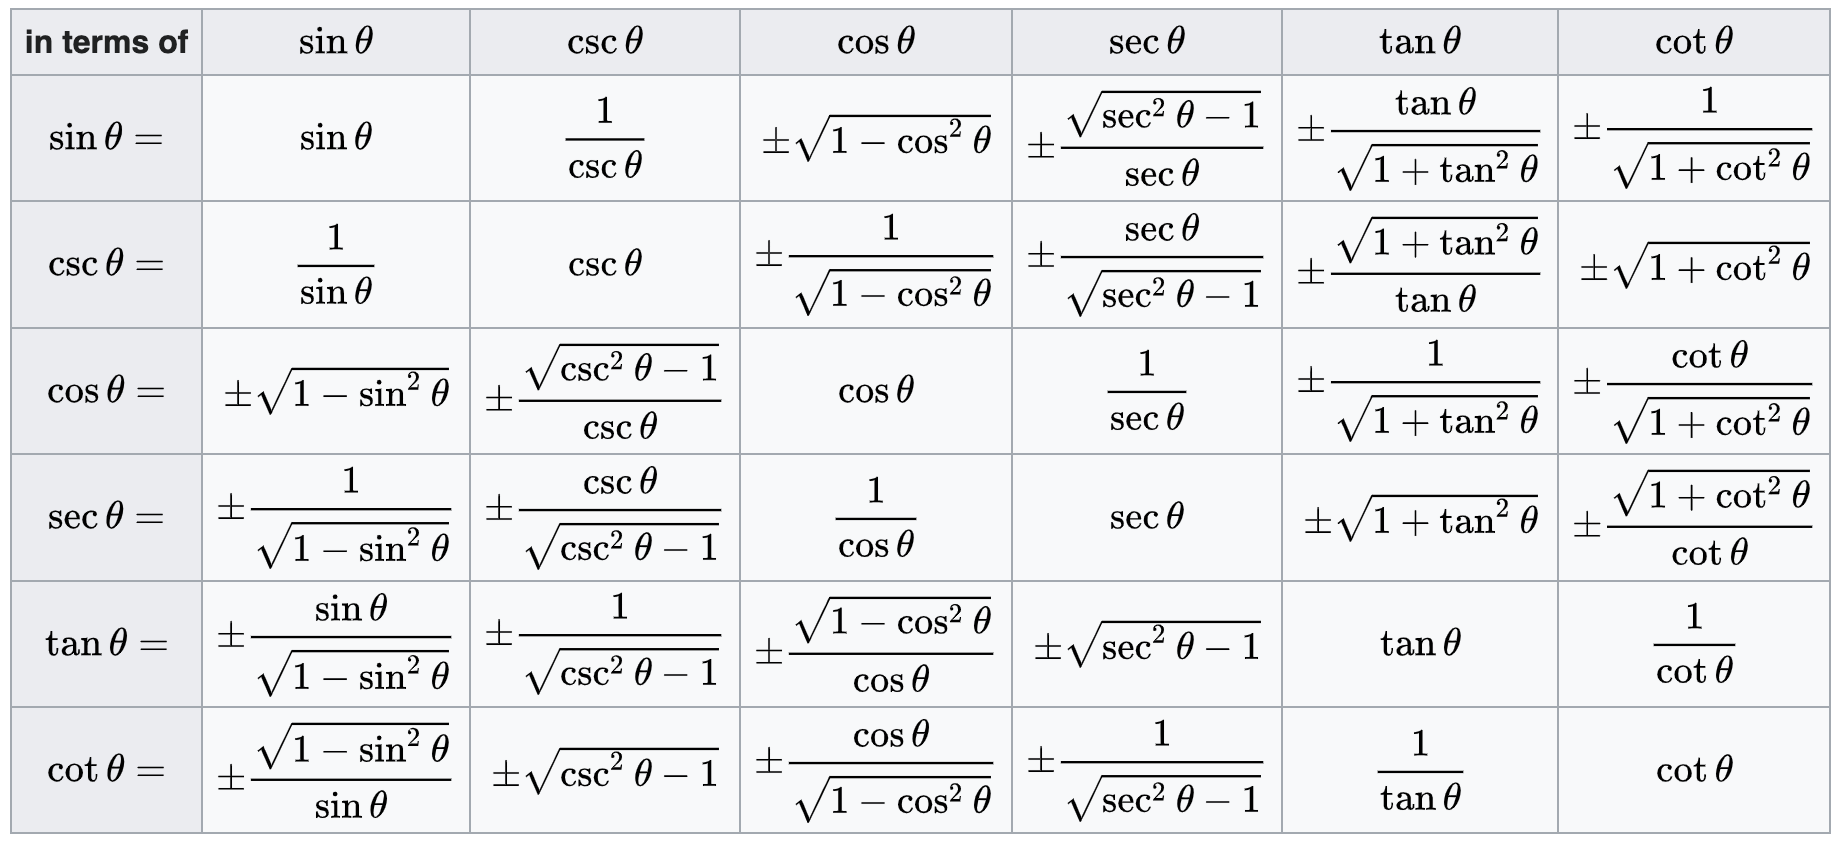
\includegraphics[width=0.8\linewidth]{../figures/trig_id.png}
  \label{fig:trig_id}
\end{figure}

På \textbf{\autoref{fig:trig_id}} ses en omregningstabel, hvor hver af de trigonometriske funktioner er givet afhængigt af hver af de 5 andre.

\subsection{Den pythagoræiske identitet (idiotformlen)}
Den pythagoræiske identitet foreskriver at
\[ 
\sin^2 \theta + \cos^2 \theta = 1
.\]

\subsection{Eksakte værdier af de trigonometriske funktioner}
\begin{figure} [ht]
  \centering
  \caption{Eksakte værdier af de trigonometriske funktioner for almindelige vinkler}
  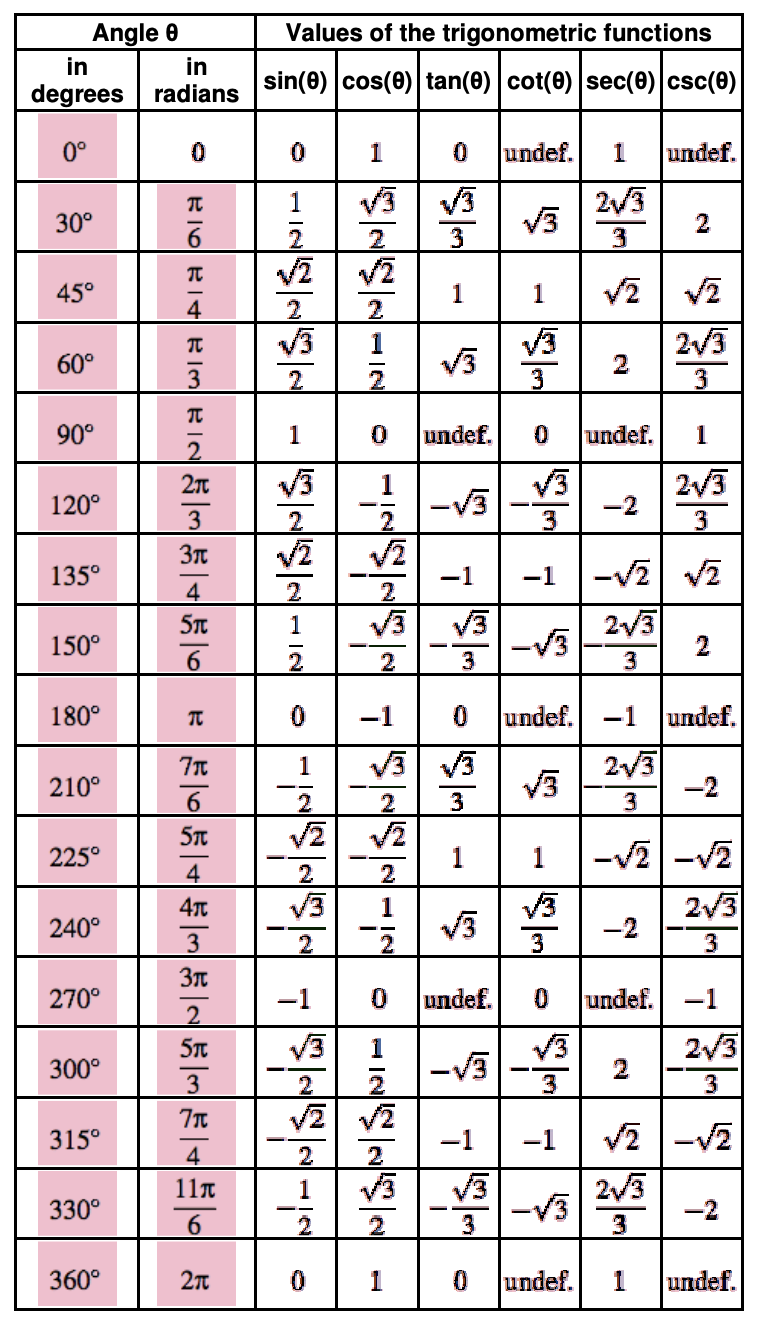
\includegraphics[width=0.75\linewidth]{../figures/trig_fun.png}
  \label{fig:trig_fun}
\end{figure}

På \textbf{\autoref{fig:trig_fun}} ses en oversigt over de eksakte værdier af de trigonometriske funktioner for de mest almindelige vinkler.

\clearpage

\subsection{Sammenligning af vinkler}
\begin{figure} [ht]
  \centering
  \caption{\textit{Cheat Sheet} til sammenligning af vinkler}
  \includegraphics[width=0.5\linewidth]{../figures/vinkelsammenligninger.png}
  \label{fig:vinkelsammenligninger}
\end{figure}

På \textbf{\autoref{fig:vinkelsammenligninger}} ses en oversigt hvilke vinkler der er ens.


\newpage


    \clearpage
    \section{Hyppigt brugte symboler til kopiering}

\begin{itemize}
  \item $\approx$
  \item $\pm$
  \item $^{\circ}$
  \item -- (langt minus til MathCad-subskript)
  \item $\neq$
  \item $\ll$
  \item $\gg$
  \item $\sim$
  \item $\mathbb{N}$
  \item $\mathbb{Z}$
  \item $\mathbb{Q}$
  \item $\mathbb{R}$
  \item $\mathbb{C}$
  \item $\ell$
  \item $\forall$
  \item $\exists$
  \item $\in$
  \item $\lor$
  \item $\land$
  \item $\implies$
  \item $\impliedby$
  \item $\iff$
  \item $\to$
  \item $\longrightarrow$
  \item $\leftrightarrow$
  \item $\uparrow$
  \item $\downarrow$
  \item $\infty$
  \item $\pm$
  \item $\mp$
  \item $\left\lceil \text{ } \right\rceil$
  \item $\left\lfloor \text{ } \right\rfloor$
  \item $\nabla$
\end{itemize}

\end{document}
